\chapter{Métrica}
\epigraphhead[50]{\epigraphtextposition{flushleftright}\epigraph{Por lo cual, atendiendo a que este género de sabandijas que llaman poetas son nuestros prójimos y cristianos —aunque malos—, viendo que todo el año idolatran mujeres y hacen otros pecados más enormes, mandamos que la Semana Santa recojan a los poetas públicos y cantoneros, como a malas mujeres y que los prediquen para convertirlos...}{Francisco de Quevedo, \textit{Premática del desengaño contra poetas güeros}}}

\section{La lengua de los poetas}
El lenguaje poético del Siglo de Oro tuvo uno de sus máximos exponentes en el teatro. La representación dramática no tenía métrica propia, sino que recurría a las formas ordinarias de la poesía común \parencite[251]{navarrotomas1991}. Por este motivo, resulta obligado abordarla de la misma manera que lo hacemos con la lírica.
 
La palabra \textit{poesía} deriva de poiesis, \textit{producción}, esto es el acto de crear. En sentido estricto, tanto la lírica como la narración y el teatro son composiciones poéticas, ya que todas ellas son actos de creación en el sentido al que se refiere la palabra \textit{poesía}. Aristóteles apunta en su \textit{Poética} (1488b20-24) que la poesía surge de nuestra predisposición para copiar y es nuestra familiaridad con el ritmo\index{ritmo} y la armonía lo que nos lleva a improvisar imitaciones. Difieren, sin embargo, en el modo en que se materializa esta creación, si se relata o se imita, si se cuenta o se enseña. No obstante, el sabio macedonio establece una relación genética entre las formas líricas y las dramáticas.

\blockquote{Y, entre los antiguos, unos fueron poetas de versos heroicos y otros de yambos [...]. Una vez aparecidas la tragedia y la comedia, los que tendían a una y a otra poesía según su propia naturaleza, unos, en vez de yambos, pasaron a hacer comedias, y los otros, de poetas épicos se convirtieron en autores de tragedias, por ser estas formas de más fuste y más apreciadas que aquellas [...]. Habiendo, pues, nacido al principio como improvisación —tanto ella como la comedia; una gracias a los que entonaban el ditirambo, y la otra, a los que iniciaban los cantos fálicos, que todavía hoy permanecen vigentes en muchas ciudades—, fue tomando cuerpo, al desarrollar sus cultivadores todo lo que de ella iba apareciendo [...]. Por otra parte, la amplitud, partiendo de las fábulas pequeñas y de una dicción burlesca, por evolucionar desde lo satírico, se dignificó tarde, y el metro se convirtió de tetrámetro en yámbico. (\poetics{1488b28-1449a-30})}

No debemos, por tanto, caer en la trampa, de confundir la poesía en general con una de sus expresiones, la lírica, como se suele hacer comúnmente, y menos con las formas externas de esta. La versificación teatral, al contrario que la lírica, no está al nivel mimético, sino que los personajes se expresan como ellos mismos, están \textit{hablando} —excepcionalmente podría estarlo si los actores\index{actor} declaman una poesía o cantan una canción, pero sería literatura dentro de la literatura; su equivalente dramático sería que los actores interpretaran a actores representando una función—. El verso se halla en la capa comunicativa entre el actor y el espectador, lo que ejemplifica de nuevo la doble enunciación del texto teatral, lo que el espectador reconoce como tal y acepta como parte de la naturaleza estética de la obra \parencite[618]{schaeffer1995}. En definitiva, la rima teatral no es mimética sino estética.

\blockquote{En el teatro de la temprana Edad Moderna las personas usan un lenguaje rimado. No me parece una cosa secundaria, de la misma manera que el lenguaje en verso y la métrica no deberían ser cosas secundarias y es triste que hoy lo sean. El lenguaje rítmico consigue en el teatro lo mismo que consiguen otros modos [...]. Se produce como una tensión entre la construcción «natural» de la oración y la forma métrica [...]. ¿Cómo afecta esto a los sentimientos del espectador? Precisamos ahora esta pregunta: ¿Cómo afecta el lenguaje oscilante según ritmos\index{ritmo} fijos en los visitantes del teatro? ¿Qué aporta el ritmo cuando se trata de que olviden los sentimientos que han traído consigo y asuman los sentimientos fingidos de los intérpretes? \parencite[p. 133; traducción propia]{aichinger2013b}}

Así pues, si hemos de distinguir entre géneros, la concepción clásica resulta particularmente apropiada para el teatro áureo porque precisamente la forma externa que suele asociarse a la lírica es un elemento destacado del drama. Sin embargo, la configuración versificada va más allá del simple adorno. Esta no solo desempeña una función estética, sino que sirve como armazón estructural, como vimos en el capítulo anterior, «la métrica tiene en el teatro del Siglo de Oro una función estructural en la que es relevante el cambio de forma métrica» \parencite[68]{arellano2007}.

Sin embargo, en su composición sonora, los versos de la poesía lírica y la dramática no difieren en lo esencial. La estructura de un poema\index{poema} puede representarse mediante relaciones numéricas, esto es, el lenguaje poético unifica lengua y números  \parencite[45]{aichinger2013b}. En otras palabras, admite ser medido y cuantificado, no en vano nos referimos a ello con el término \textit{metro}.

¿Pero qué es lo que medimos? Esta es la primera cuestión que hemos de resolver antes de embarcarnos en una mensura. Empezaremos para ello por el elemento mínimo, que es el verso. Caramuel indica que \blockquote{los Poemas se componen de estrofas; las Estrofas de versos; los Versos de Palabras; las Palabras de Sílabas, y estas finalmente de Letras. Así, la mínima parte del Poema es la letra} \parencite[p. 35; mayúsculas en el original]{caramuel2007}. No obstante, debemos precisar esto. La \textit{letra} de Caramuel —nosotros la llamaríamos hoy \textit{fonema}— no asume una función aislada, ya que es incapaz de crear un ritmo\index{ritmo} si no es en combinación con otros sonidos. La palabra sí podría hacerlo, aunque no necesariamente, en tanto que para ello se necesita un número mínimo de sílabas que no todas las palabras reúnen. De esta manera, la unidad mínima del poema\index{poema} es el verso, si bien este puede descomponerse en unidades menores pero insuficientes para constituir poemas. Más adelante, veremos cómo se agrupan. Una vez tenemos nuestro objeto de estudio, debemos determinar las unidades en función de las cuales asignaremos el valor a la medida de una magnitud. Aquí hemos de detenernos para considerar una particularidad de la lengua española. Debemos retrotraernos a la poética clásica, surgida en el ámbito de lenguas de ritmo acentual\index{lengua!de ritmo acentual} como el latín y el griego, basadas en la cantidad como ocurre hoy, por ejemplo, con el inglés \parencite[21]{quilis2013}.
\blockquote[{\cite[307]{bello1981}}]{Había sílabas \textit{breves} o de rápida pronunciación, y otras \textit{largas}, a manera de notas sostenidas, y por el tiempo que se gastaba en pronunciarlas, estaban las segundas con respecto a las primeras, que daban el tipo, en la proporción aproximada de 1 a 2.
		
Seguramente los griegos y romanos al hablar, gozábanse en pronunciar con prolongado aliento las sílabas largas, y velozmente las breves, de un modo aproximado a lo que se practica en el canto gregoriano, y en los recitados de la ópera, aunque no extremando lo largo y breve, sino atemperando lo uno a lo otro, en la proporción de 1 a 2, y dentro de los límites naturales del aliento sonoro.}
Por este motivo, la unidad de las poéticas clásicas es el pie métrico\index{pie métrico}. Lo que hace un hexámetro es estar compuesto de seis pies métricos. La lengua española, al contrario que aquellas, es de ritmo silábico\index{lengua!de ritmo silábico}, por lo que su versificación ha de adaptarse a su naturaleza \parencites[20]{herrero1996}[27-30]{torre1999}[21]{quilis2013}. Esto dota al verso español de unas características peculiares y diferenciada de los propios de otras lenguas de ritmo acentual \parencite[54-55]{cantero2002}, si bien no han faltado los intentos de ilustrísimas plumas por trasladarlo \parencite{dfernandez2021}. La consecuencia más importante de esto es que el metro castellano no lo medimos en pies sino en sílabas. En palabras de Navarro~Tomás~\parencite*[34]{navarrotomas1991}, \blockquote{aplicar al estudio de una métrica extranjera el criterio de los hábitos adquiridos en la lengua propia es situarse en un equivocado punto de vista}. El prurito clasicista de \citeauthor{diazrengifo2012}~\parencite*[174]{diazrengifo2012} le lleva a contemplar la cantidad, solo para, de inmediato, igualarla con el acento y señalar este como única distinción válida. No obstante, es usual que se intercalen pasajes de ritmo acentual en el teatro áureo porque incluye a menudo partes cantadas. En ocasiones, estos fragmentos dejan intuir su naturaleza métrica en ciertos indicios, como la irregularidad en el número de sílabas, que queda compensada por el ritmo acentual \parencite[416-417]{torrente2016}. Desafortunadamente, incluso estando dispuestos a poner el pie en el terreno de los musicólogos y tratar cada estrofa cantada de manera individual, la tarea resultaría probablemente fútil debido a la escasez de las fuentes (pp. 323-324).

 Por otra parte, la sílaba métrica tiende a corresponderse con su realización fonética —sea esta el fruto de una licencia poética o del normal uso del lenguaje— más que a una expresión fonológica idealizada de un segmento aislado \parencite[53]{dominguez2014a}. La poesía se aprovecha de esa característica para introducir accidentes suprasegmentales, como la sinalefa o la diéresis, ubicuos en el texto en verso como medio de ajuste silábico \parencite[55-59]{dominguez2014a}. Así, para abordar el teatro aurisecular, hay que considerar el metro según su silabación fonética y tratar las irregularidades considerando los medios de compensación métrica. Por fortuna, las reglas de la división silábica del español son claras \parencite{hualde1991}, lo que simplifica la tarea de sistematizarlas en un programa informático. Ya discutimos estos fenómenos en el capítulo dedicado a presentar los fundamentos teóricos de la aproximación fonológica. Por lo tanto, daremos por supuestas también en la métrica esas nociones.
 
La sílaba del metro español se caracteriza por la presencia o ausencia de acento, y esta propiedad lo faculta para determinar la configuración rítmica del verso. Esto es, entendemos el verso como una serie de sílabas que adoptan un valor binario: tónica/átona. La distribución de estos valores puede responder a un patrón determinado, si bien este no resulta absolutamente necesario. En otras palabras, la única regla fija es que el último acento de un verso $n$-sílabo va sobre la sílaba $n-1$, a partir de la cual no se consideran las sílabas inacentuadas, pero, dependiendo del tipo de verso, los acentos suelen recaer en determinadas posiciones. Así, por ejemplo, una característica habitual de los versos endecasílabos\index{verso!endecasílabo} es emplazar un acento en la sexta sílaba. Sin embargo, no ocurre igual en, por mencionar algunos, los sáficos puros o los de gaita gallega. Asimismo, existen otros acentos facultativos que caracterizan un tipo de verso. Por ejemplo, un verso heroico puro lleva acentos en la segunda, sexta y décima sílaba. Adicionalmente, el endecasílabo heroico admite otros acentos en la cuarta y la octava, de cuyas combinaciones dependerá que sea pleno, corto o largo.

Debemos advertir que en los textos teatrales existe una excepción a lo dicho. Muchas obras incluyen versos cantados que, como es lógico, no se atienen a la prosodia española sino a la musical. Por lo tanto, sería posible alargar o acortar sonidos, juntar o desdoblar sílabas. En estos casos, el texto tendría más que ver con los ritmos acentuales que con el silábico castellano, pero no podrían conocerse a ciencia cierta los pies que lo constituyen. Sin otra indicación que la letra, sin conocer la música, no cabe hacer más que conjeturas.

\section{Elementos métricos}
Como dijimos, el verso es la unidad poética mínima y, por lo tanto, qué más apropiado que comenzar por él. Navarro~Tomás~\parencite*[34-35]{navarrotomas1991} lo define como «una serie de palabras cuya disposición produce un determinado efecto rítmico». Este efecto, dice, se fundamenta en los acentos producidos al espirar las palabras. En la lengua española, el tono o la cantidad no tienen relevancia rítmica. Otros elementos, como la armonía vocálica o la aliteración\index{aliteración}, solo sirven, a lo sumo, de refuerzo, ya que no tienen capacidad de alterar el ritmo\index{ritmo}, mientras que el acento por sí mismo es suficiente para definirlo. Además de los acentos que moldean el verso, las sílabas y pausas marcan sus límites y divisiones internas. En cualquier caso, para considerar un verso como una unidad rítmica independiente, este ha de tener cuatro o más sílabas.

El verso español se atiene a la métrica románica y, como tal, sus elementos constitutivos elementales son el \textit{acento de intensidad}\index{acento}, la \textit{pausa métrica}\index{pausa} y el \textit{cómputo silábico}\index{cómputo silábico} \parencite[22]{baehr1997}. A partir de estos componentes básicos es como se construye el resto. Aquellos que no derivan directamente de ellos pueden ser complementarios pero no determinantes.

La poesía tiene raíces musicales. De esta manera, los acentos del verso se distribuyen formando un patrón rítmico. Según Navarro Tomás \parencite*[35-36]{navarrotomas1991}, además del acento final, el verso poseería necesariamente otro apoyo rítmico al comienzo. El \textit{periodo rítmico}\index{periodo rítmico!interior} \textit{interior} sería así la porción del verso comprendida entre la sílaba que recibe el primer apoyo rítmico  hasta la que antecede al último acento. Las sílabas átonas que preceden al primer apoyo rítmico actuarían como anacrusa\index{anacrusa} o antecompás. El \textit{periodo de enlace}\index{periodo rítmico!de enlace} comenzaría, por su parte, en la última sílaba acentuada del verso\index{cumbre tonal}, las sílabas que la sigan, la pausa al final del verso y, si las hubiera, las sílabas en anacrusa del verso siguiente (\ref{ex:periodo}). Estos dos periodos se repetirían periódicamente al modo de las composiciones musicales.

\begin{exe}
	\ex\label{ex:periodo}$\overbrace{Je-ru-sa}^{Anacrusa}-\overbrace{l\acute{e}n\ las\ rui-nas\ del\ cal}^{Periodo\ r\acute{i}tmico}-\overbrace{de-o}^{Enlace}.$\\
	\strut\hfill(Moreto, \citetitle[124]{moreto2018})
\end{exe}

Los periodos se organizan en \textit{cláusulas}\index{cláusula} de dos o tres sílabas, cuyo equivalente en las lenguas de ritmo acentual\index{lengua!de ritmo acentual} es el pie métrico. No debe confundirse con este porque, como indicamos, la cláusula española es acentual y no cuantitativa. Todas las cláusulas de los versos españoles son disilábicas o trisilábicas. Las primeras son de ritmo \textit{trocaico} si el acento recae en la primera o \textit{yámbicas} si lo hace sobre la segunda. En cuanto a las cláusulas trisílabas, serán \textit{dactílicas} si el acento recae en la primera sílaba, \textit{anfibráquicas} si en la segunda y \textit{anapésticas} si es en la tercera \parencite[141-142]{bello1981}. Navarro~Tomás~\parencite*[37]{navarrotomas1991} nota que la interpretación del pie es subjetiva; lo ilustra con, entre otros, el primer verso del celebérrimo poema\index{poema} de Bécquer «De salón en el ángulo oscuro». Lo mismo sucede con el verso del ejemplo \ref{ex:salon}, que se lee tanto como anapéstico (\ref{ex:salon1}) como dactílico con anacrusa (\ref{ex:salon2}).
\begin{exe}
	\ex\label{ex:salon}\textit{Caminad, caminad a la sombra}
	\begin{xlist}
		\ex\label{ex:salon1}\texttt{--+|--+|--+|-||}
		\ex\label{ex:salon2}\texttt{--|+--|+--|+-||}
	\end{xlist}
\strut\hfill(Calderón, \citetitle[1390]{calderon_viatico})
\end{exe}

Esto ofrece ya una primera pista de que el modelo de periodo rítmico de Navarro Tomás presenta algunos puntos problemáticos. Nos detendremos en ellos más adelante.

La \textit{cantidad silábica}\index{cantidad silábica}, si bien no se tiene en cuenta como medida del metro, tampoco es una magnitud inexistente en español, a pesar de no tener la relevancia de la que goza en otros sistemas métricos. Las sílabas tienen diferente duración, como se aprecia en los sonogramas\index{sonograma}. Esto suele compensarse en las cláusulas, cuya duración suele ser más uniforme, especialmente cuando se trata de dos del mismo tipo, de forma que estas se ajustan al compás \parencite[37]{navarrotomas1991}. Este fenómeno carece de expresión a nivel fonológico y en la declamación se compensa alterando la realización de los sonidos para ajustar el periodo. Por este motivo, lo mencionamos aquí, pero no lo tendremos en cuenta para la parte práctica del trabajo, que, después de todo, es un modelo fonológico que no aspira a representar exactamente el sonido físico.

A los elementos rítmicos fundamentales hay que añadir otros que, sin tener una función estructural, contribuyen a realzar los componentes básicos y aumentar la eufonía del verso. Podemos contar entre estos, por ejemplo, las aliteraciones, la simetría, la anáfora, el \textit{lexaprén}, \textit{macho e femea} y el \textit{manzobre} \parencite[126-129]{dominguez2014a}.

Los versos se clasifican atendiendo a varios criterios, en los que influye tanto el cómputo silábico como la posición de los acentos. Llamamos \textit{métricos} a los versos que tienen un número fijo de sílabas y \textit{amétricos} a los que no. Si los periodos del verso se distribuyen según una estructura prefijada, el verso será \textit{monorrítmico} y  será \textit{polirrítmico} si esta disposición varía. Entre los versos amétricos, son \textit{acentuales} aquellos compuestos por un número variable de cláusulas del mismo tipo, de modo que el ritmo\index{ritmo} se mantiene, mientras que serán \textit{libres} los que no siguen un patrón. En el término medio entre ambos, se hallan los versos \textit{fluctuantes} \parencite[39]{navarrotomas1991}. Al final de cada verso hay una \textit{pausa}\index{pausa} y, en versos compuestos, hay además otra interna. Las pausas van precedidas de terminación oxítona, paroxítona o proparoxítona \parencite[39-40]{navarrotomas1991}.

La rima, aunque usada con muchísima cautela en la poesía clásica culta, abundaba en las canciones populares latinas. Sin embargo, su auge llegó en la Edad Media y, sobre todo, con la trova, que tomó la rima consonante como una de las máximas expresiones de su arte. La asonancia quedó relegada a las formas populares, pero cobró importancia en algunos géneros típicamente españoles \parencite[40-41]{navarrotomas1991}. 

La agrupación de versos encuentra una unidad de orden superior en la estrofa\index{estrofa}. Además, la estructura del verso se apoya ocasionalmente en determinados recursos facultativos. El poeta tiene libertad para jugar con la distribución de las palabras y producir efectos como repeticiones o paralelismos. También disfruta la potestad de hacer corresponder las vocales en el interior del verso, particularmente aquellas en posición acentuada, de manera que se produzca una armonía vocálica o adaptar los sonidos consonánticos para evocar emociones que convengan al verso \parencite[41-42]{navarrotomas1991}.

\section{Ritmo}\index{ritmo}

El ritmo de un verso depende de sus acentos. El acento es un realce sonoro en determinadas sílabas para hacerlas destacar sobre el resto en los segmentos de lengua hablada. El primer tipo de acento que encontramos al escuchar hablar español es el \textit{prosódico}\index{acento!prosódico}. Sin embargo, debemos matizar aquí su carácter, en función del grado de complejidad de la verbalización. Así, si estamos tratando una palabra aislada, está llevará siempre un acento prosódico en mayor o menor medida, el acento  \textit{léxico}\index{acento!léxico}. Si, por el contrario, la palabra se halla en contexto, se distingue entre palabras tónicas y átonas. Este acento del habla normal también se mantiene en la pronunciación del verso, salvo en contadas ocasiones donde el poeta se concede una licencia para cuadrar el metro \parencite[24]{baehr1997}.

\blockquote[{\cite[174-175]{diazrengifo2012}}]{Acento es un sonido con que herimos y levantamos más una sílaba cuando la pronunciamos y nos detenemos más en aquella que en cualquiera de las otras de un mismo vocablo, como cuando decimos «agúdo», «poéta», herimos la «u» y la «e» y las levantamos sobre todas las otras sílabas. Y hablo aquí solamente del acento que predomina en cada dicción, no del grave o del circunflejo que ponen los latinos, los cuales nos conciernen poco para lo que al presente tratamos. Este acento predominante no puede ser más que uno en cada vocablo, ni se puede hallar sino en la sílaba última, como «perdí», «gané»; o en la penúltima, como «máno», «sagráda»; o en la antepenúltima, como «próspero», «alhóndiga». Llamo sílaba última la postrera de cada dicción; penúltima, la más cercana a la última; y antepenúltima, la que es tercera comenzando de la última. Supuesto este fundamento, aquella sílaba es larga que se pronuncia con el acento predominante, y todas las demás que estuvieren delante o se siguieren después della en un mismo vocablo serán breves, como en «caballéro» la «e» es larga y las demás breves, en «dignísimo» la «ni» es larga, las demás breves. Entre las que están delante contamos muchas dicciones de una sílaba, las cuales no tienen acento predominante, sino que son breves como las demás del vocablo a quien se arriman, como «la», «lo», «me», «te», «se», «sin», «con», «a», «de», «por», «en», etc. Así como «en vida con ampáro», la «en» y la «con» no tienen acento por sí, sino son breves como las demás a quien se ayuntan. Podría decir alguno que corre en «dignísimo» la  «si» que no la «di», y lo mismo parecerá en todos los vocablos que tuvieren el acento en la antepenúltima. Pero no es así, antes todas son iguales; y la causa de parecer aquella más breve que las otras es el haber precedido inmediatamente la larga, en la cual, como se subió la voz, cuando baja a la breve que se sigue, parece que se despeña y que corre más por ella que por las otras, como en realidad en todas gaste un mismo tiempo.}

Como ya apreció Díaz Rengifo, el acento prosódico depende del tipo de palabra y su origen histórico. Las observaciones del tratadista son certeras en tanto que, efectivamente, las preposiciones y los pronombres que funcionan como complemento verbal no preposicional son inacentuadas —de ahí que los últimos reciban el nombre de \textit{pronombres átonos}—, mientras que, por el contrario, los sustantivos\index{sustantivo} sí llevan acento \parencite[22-26]{quilis2013}. Este además recae en la última, penúltima o antepenúltima sílaba de la palabra. De esta manera, cada una lleva un solo acento prosódico, con la excepción de los adverbios terminados en \textit{-mente}\index{adverbio!{en -mente}@{en -\textit{mente}}} \parencite{quilis2013}. No llama la atención que, ya a finales del siglo \textsc{xvi}, hubiera sido descrito el sistema con gran precisión, de forma que el mismo concepto se ha ido transmitiendo hasta las poéticas contemporáneas sin experimentar cambios cualitativos sustanciales.

Esto\index{acento!contiguo} es una generalización aplicable a la mayoría de los casos. En realidad, las marcas acentuales presentan diferencias sutiles y podría hablarse de una gradación del acento con diferentes niveles \parencite[173]{navarrotomas2004}. Así, cuando concurren varios acentos contiguos, algunas de las sílabas tónicas pierden sonoridad, lo que Paraíso \parencite[81]{paraiso2000} denomina «desacentuación rítmica secundaria». Esto justifica, por ejemplo, la taxonomía del octosílabo\index{verso!octosílabo} de Navarro~Tomás~\parencite*[p. 64 y ss.]{navarrotomas2014a}, que veremos más adelante. El caso contrario también se cumple: una serie de sílabas inacentuadas tampoco tiene un nivel de intensidad uniforme.

Debemos advertir, no obstante, que los acentos contiguos\index{acento!contiguo} también se emplean como \textit{acento enfático}\index{acento!enfático}, un recurso expresivo \parencite[83-84]{paraiso2000}. En el texto dramático esto se hace más evidente si cabe. Piénsese en una serie de réplicas y contrarréplicas monosilábicas como las del ejemplo \ref{ex:contiguos}, con un ritmo \texttt{++-++++}.

\begin{exe}
	\ex\label{ex:contiguos}\textsc{Erífila}\hspace{1cm}Yo digo tal.\\
	\textsc{Leonato}\hspace{2cm}Sí.\\
	\textsc{Erífila}\hspace{3cm}¿Yo?\\
	\textsc{Leonato}\hspace{4cm}Sí.\\
	\strut\hfill(Lope de Vega, \nocite{vegavalencia}\textit{Los locos de Valencia}, v. 233)
\end{exe}

En este caso, no parece sensato reducir los acentos sobre las tablas, sino más bien todo lo contrario, que cada actor pronuncie su línea realzando la intensidad para adecuarse a lo que demanda la acción, a despecho del ritmo ideal que pudiera tener el verso. Por ese motivo, solo consideraremos las reducciones \textit{a posteriori}, como una posibilidad adicional de clasificación. Por el contrario, un único recitador se encontraría en dificultades para reproducir el diálogo a la manera de dos actores\index{actor} contando con solo un aparato fonador.

La cuestión necesita ser investigada en detalle, pues implica aspectos estilísticos, semánticos, fonológicos e incluso fonéticos \parencite[57-58]{sanchez2017}. \citeauthor{sanchez2017} se aviene a partir de los acentos gramaticales entretanto como solución de compromiso. Nosotros optaremos por lo mismo: se trata de definir un modelo que, incompleto, igual que todos, no abarca la totalidad del objeto de estudio; sin embargo, esa limitación facilita concentrarse en una de sus facetas\index{acento!contiguo}.

\subsection{Palabras acentuadas e inacentuadas}
En la parte práctica necesitaremos determinar qué palabras del verso portan acento métrico.Nos guiaremos, pues, por ciertas reglas gramaticales para distinguirlas. Esta sección presenta tanto esas reglas y sus excepciones.

En español, las palabras solo tienen una sílaba acentuada \parencite[22]{quilis2013}, con excepción de los adverbios\index{adverbio!{en -mente}@{en -\textit{mente}}} terminados en \textit{-mente} (\ref{ex:mente}), que contienen dos sílabas tónicas \parencite[26]{quilis2013}\footnote{Emplearemos la notación \texttt{+} para las sílabas acentuadas y \texttt{-} para las inacentuadas, en lugar de los símbolos de breve y larga, que no describen propiedades de la sílaba española.}. El resto de los adverbios\index{adverbio} se acentúan una sola vez (\ref{ex:adv}), salvo cuando cumplen otra función, pues ahí serán son átonos en algunas ocasiones. Un caso especial es \textit{tanto} y su forma apocopada \textit{tan}, ya que la primera es tónica y la segunda átona \autocite[169a]{navarrotomas2004}. También es irregular \textit{medio}, puesto que es inacentuada cuando actúa como adverbio (\ref{ex:medio1}), si bien es tónica (\ref{ex:medio2}) como adjetivo\index{adjetivo} \autocite[169c]{navarrotomas2004}.
\begin{exe}
	\ex\label{ex:mente} \textit{so·la·men·te} \tab \texttt{+-+-}
		\ex\label{ex:adv} \textit{so·lo}\tab \texttt{+-}
		\ex\label{ex:medio1} \textit{me·dio bo·rra·cho}\tab \texttt{--|-+-}
		\ex\label{ex:medio2} \textit{me·dio li·tro}\tab \texttt{+-|-+-}
\end{exe}

El verbo\index{verbo} es la única clase verbal que va siempre acentuado en todas sus modalidades \parencite[166]{navarrotomas2004}. Además de cuando es predicativo, también es tónico en sus funciones semipredicativas o copulativas (\ref{ex:es}), incluso en su función auxiliar (\ref{ex:ha}).
\begin{exe}
	\ex\label{ex:es}\textit{es sue·ño}\tab \texttt{+|+-}
	\ex\label{ex:ha}\textit{ha di·cho}\tab \texttt{+|+-} 
\end{exe}

Las formas nominales\index{sustantivo} suelen ser también palabras acentuadas en español (\ref{ex:tomas}, \ref{ex:santo}) salvo en excepciones concretas \parencite[167]{navarrotomas2004}. Estas irregularidades ocurren en las fórmulas de tratamiento como \textit{don} o \textit{fray} antepuestas al nombre (\ref{ex:santotomas}), la primera parte de una expresión vocativa\index{vocativo} compuesta (\ref{ex:santodios}), en caso de nombres compuestos, aquellos que anteceden al último (\ref{ex:josetomas}), nombres prepositivos (\ref{ex:santodeldia})
\begin{exe}
	\ex\label{ex:tomas} \textit{To·más}\tab \texttt{-+}
	\ex\label{ex:santo} \textit{el san·to}\tab  \texttt{-|+-}
	\ex \textit{San·to To·más}\tab  \texttt{--|-+}\label{ex:santotomas}
		\ex\label{ex:santodios} \textit{¡San·to Dios!}\tab \texttt{--|+}\footnote{En este caso, en alternancia con el ritmo ordinario (\texttt{+-|+}) si se enfatiza la primera sílaba.}.
	\ex \textit{Jo·sé To·más}\tab  \texttt{--|-+}\label{ex:josetomas}
	\ex \textit{santo del día}\tab \texttt{--|-|+-}\label{ex:santodeldia}
\end{exe}

Las preposiciones\index{preposición} son átonas (\ref{ex:a}) excepto \textit{según}, con independencia de su función \parencite[170]{navarrotomas2004}. 
\begin{exe}
	\ex\label{ex:a} \textit{a ca·sa} \tab \texttt{-|+-}
\end{exe}

Los artículos\index{artículo} determinados son inacentuados (\ref{ex:el}), al contrario que los indeterminados, que son tónicos (\ref{ex:un}). Constituyen una excepción estos últimos  \parencite[170]{navarrotomas2004} cuando sirven para dar una valoración aproximativa (\ref{ex:unos}).
\begin{exe}
	\ex\label{ex:el}\textit{el hom·bre}\tab \texttt{-|+-}
	\ex\label{ex:un}\textit{un hom·bre}\tab \texttt{+|+-}
	\ex\label{ex:unos}\textit{u·nas tres ho·ras}\tab \texttt{--|+|+-}
\end{exe}

Los adjetivos\index{adjetivo} léxicos, esto es, los calificativos (\ref{ex:adj1}) y relacionales (\ref{ex:adj2}) llevan acento, no así todos los de las clases cerradas adjetivales. Los indefinidos son acentuados, pero el distributivo \textit{cada} suele tener una relación átona \parencite[168.f]{navarrotomas2004}
\begin{exe}
	\ex\label{ex:adj1}\textit{san·to se·cre·to}\tab \texttt{+-|-+-}
	\ex\label{ex:adj2}\textit{co·ro·na im·pe·rial}\tab \texttt{-+-|--+}
\end{exe}

Otro tipo de palabras con uso adjetivo\index{adjetivo} varían según el caso. De esta manera, los numerales\index{numeral}, tanto ordinales como cardinales, son siempre tónicos por sí mismos (\ref{ex:num1}). Sin embargo, al igual que ocurre con los sustantivos\index{sustantivo}, el acento recae en el último elemento si estos constituyen una serie, siendo los precedentes átonos (\ref{ex:num2}). Lo mismo sucede si desempeñan una función nominal (\ref{ex:num3}).
\begin{exe}
	\ex\label{ex:num1}\textit{pri·mer pre·mio}\tab \texttt{-+|+-}
	\ex\label{ex:num2}\textit{trein·ta mil}\tab  \texttt{--|+}
		\ex\label{ex:num3}\textit{el trigésimo noveno}\tab  \texttt{-|----|-+-}
\end{exe}

Los demostrativos\index{demostrativo} son siempre tónicos, tanto en su función pronominal como adjetival.
\begin{exe}
	\ex \textit{es es·te}\tab \texttt{+|+-}
	\ex \textit{es·te tex·to}\tab \texttt{+-|+-}
\end{exe}

El acento varía en los posesivos\index{posesivo} dependiendo de su función. Si actúan como determinante (\ref{ex:nuestro1}), son definidos \parencite[18.2.1a]{rae2010a} y, como los personales, también átonos. Por el contrario, serán tónicos si desempeñan una función adjetival (\ref{ex:nuestro2}). Esto se deduce de la posición porque, en función determinativa, el posesivo ocupa una posición prenominal, mientras que es posnominal en función adjetival \parencite[18.2.2g]{rae2010a}.
\begin{exe}
	\ex\label{ex:nuestro1}\textit{nues·tro re·me·dio}\tab \texttt{--|-+-}
	\ex\label{ex:nuestro2}\textit{re·me·dio nues·tro}\tab \texttt{-+-|+-}
\end{exe}

Las partículas exclamativas\index{exclamativo} e interrogativas\index{interrogativo} son tónicas (\ref{ex:int1}), pero su contrapartida relativa\index{relativo} es átona (\ref{ex:int2}).
\begin{exe}
	\ex\label{ex:int1}\textit{¿Cuán·do vie·nes?}\tab\texttt{+-|+-}
	\ex\label{ex:int2}\textit{Cuan·do ven·ga.}\tab\texttt{--|+-}
\end{exe}

Los pronombres personales\index{pronombre} son tónicos en el caso nominativo (\ref{ex:yo}) y en el oblicuo (\ref{ex:mi}) y átonos en dativo (\ref{ex:le}) y acusativo (\ref{ex:lo}). Los pronombres reflexivos también son átonos  (\ref{ex:se}). En los pronombres recíprocos con desambiguación, serán tónicos o no obedeciendo a las reglas de sus componentes, esto es, el componente reflexivo (\textit{nos}, \textit{os}, \textit{se}) será átono mientras que tanto el nominativo como el oblicuo (incluyendo \textit{sí} para la tercera persona) o adjetival (\textit{mismo}) serán tónicos.
\begin{exe}
	\ex\label{ex:yo}\textit{él vie·ne}\tab\texttt{+|+-}
	\ex\label{ex:mi}\textit{pa·ra mí}\tab\texttt{--|+}
	\ex\label{ex:le}\textit{le da al·go}\tab\texttt{-|+|+-}
	\ex\label{ex:lo}\textit{lo co·ge}\tab\texttt{-|+-}
	\ex\label{ex:se}\textit{se pei·na}\tab\texttt{-|+-}
\end{exe}

Son átonas, según Quilis~\parencite*[24]{quilis2013}, las conjunciones copulativas (\ref{ex:y}), disyuntivas (\ref{ex:o}), la polivalente \textit{que} (\ref{ex:que}), adversativas (\ref{ex:pero}), causales (\ref{ex:pues}), consecutivas (\ref{ex:conque}), condicionales (\ref{ex:cuando}) y concesivas (\ref{ex:aunque}). No obstante, pueden ser tónicas en función adverbial (\ref{ex:yesto}). Constituyen la excepción las disyuntivas \textit{ora}, \textit{ya} y \textit{bien} (\ref{ex:ora}), la consecutiva \textit{así} (\ref{ex:asi}) y la temporal \textit{apenas}, así como las compuestas adversativas (\ref{ex:noobstante}), temporales (\ref{ex:nobien}), condicionales (\ref{ex:contalque}) y concesivas  (\ref{ex:malque}).
\begin{exe}
	\ex\label{ex:y}\textit{ni u·no ni o·tro}\tab \texttt{-|+-|+-}
	\ex\label{ex:o}\textit{él o yo}\tab \texttt{+|-|+}
	\ex\label{ex:que}\textit{da·le que te pe·go}\tab \texttt{+-|-|-|+-}
	\ex\label{ex:pero}\textit{sí, pe·ro no}\tab \texttt{+|--|+}
	\ex\label{ex:pues}\textit{pues·to que te gus·ta, qué·da·te·lo}\tab \texttt{--|-|-+-|+---}
	\ex\label{ex:conque}\textit{ya tie·nes lo tu·yo, con·que ve·te}\tab \texttt{+|+-|-|+-|--|+-}
	\ex\label{ex:cuando}\textit{si pue·des, llá·ma·me}\tab \texttt{-|+-|+--}
	\ex\label{ex:aunque}\textit{no lo creeré aunque lo vea}\tab\texttt{+|-|--+|--|-|+-}
	\ex\label{ex:yesto}\textit{¿Y esto?}\tab \texttt{+|+-}
	\ex\label{ex:ora}\textit{ora unos, ora otros}\tab \texttt{+-|+-|+-|+-}
	\ex\label{ex:asi}\textit{no co·rre·rí·a a·sí lo fus·ti·ga·ran}\tab \texttt{+|--+-|-+|-|--+-}
	\ex\label{ex:noobstante}\textit{a·rre·gla·da no obs·tan·te in·for·mal}\tab \texttt{--+-|+|-+-|--+}
	\ex\label{ex:nobien}\textit{se mar·chó no bien lle·gó}\tab \texttt{-|+-|+|+|-+}
	\ex\label{ex:contalque}\textit{haz·lo con tal que fun·cio·ne}\tab\texttt{+-|-+-|-+-}
	\ex\label{ex:malque}\textit{a·cep·to mal que me pe·se}\tab\texttt{-+-|+|-|-|+-}
\end{exe}

Los adverbios\index{adverbio} empleados en función conjuntiva (\ref{ex:luego}) o como parte de una locución conjuntiva \parencite[31.6.1b]{rae2010a} se rigen por la regla general de la conjunción (\ref{ex:mas}) y, por lo tanto, son átonos \parencite[]{navarrotomas2004}.
\begin{exe}
	\ex\label{ex:luego} \textit{pien·so, lue·go e·xis·to}\tab\texttt{+-|--|-+-}
	\ex\label{ex:mas} \textit{no ha·ce más que lo que de·be}\tab\texttt{+|+-|-|-|-|-|+-}
\end{exe}

Aquí identificamos un patrón considerando las conjunciones a partir de sus componentes individuales. Aquellas compuestas de palabras que individualmente son átonas serán asimismo átonas, mientras que otras que contengan una palabra que por sí misma es tónica conservarán normalmente su acento. De este modo, en las adversativas compuestas, \textit{en tanto} conserva el acento en su segunda sílaba por ser tónica, pero \textit{en cuanto} es átona en todas sus sílabas.

\subsection{Acento métrico}
Además del acento prosódico, para caracterizar el ritmo\index{ritmo} adecuadamente hay que tener en cuenta el \textit{acento métrico}\index{acento!métrico} o \textit{rítmico}\index{acento!rítmico|see {acento métrico}}. Se define este acento como los golpes tónicos intrínsecos al ritmo particular de un verso. De acuerdo con \citeauthor{baehr1997}~\parencite*[8-9]{baehr1997}, en cada verso se hallan como mínimo dos acentos rítmicos, uno al final del verso en la rima y otro que varía su posición entre las cuatro primeras sílabas. Los acentos prosódicos no se traducen siempre en acentos métricos ni viceversa.

El verso español puede reproducir patrones rítmicos, aunque no necesariamente. Los versos endecasílabos\index{verso!endecasílabo} (\Cref{tab:endecasilabos}), por ejemplo, se prestan a que el poeta aplique ciertos patrones para obtener un efecto estético de manera que, aparte del acento fijo en la décima sílaba, suele acentuar la sexta sílaba en la mayoría de los casos, pero un tercer acento facultativo en las cuatro primeras sílabas determina si el verso es enfático, heroico, melódico o sáfico, o incluso otro tipo de verso menos frecuente con otras combinaciones \parencite[22]{quilis2013}. Los octosílabos\index{verso!octosílabo} áureos, por su parte, tienden a seguir un ritmo\index{ritmo} trocaico, dactílico o una de dos combinaciones de estos \parencites[93-94]{torre2000}[274-275]{navarrotomas1991}. La realización del ritmo métrico, sin ser del todo coincidente con los acentos prosódicos, suele estar determinada por estos \parencite[26]{baehr1997}, por lo que sería posible deducirla a partir de la prosodia. 

De la misma manera que los versos endecasílabos\index{verso!endecasílabo} se clasifican tradicionalmente en categorías según la posición de los acentos métricos, otros tipos de verso también se categorizan de forma análoga. En el caso del octosílabo\index{verso!octosílabo}, el más común en el teatro áureo, hay clasificaciones, como las de Navarro Tomás~\parencite*[64 y ss.]{navarrotomas2014a} o \citeauthor{varela2005}~\parencite*[149-158]{varela2005}. Para el primero, los versos octosílabos podrían reducirse las sesenta y cuatro combinaciones rítmicas posibles de entre uno y siete acentos a tan solo cuatro clases métricas (\Cref{tab:octosilabos}): trocaica (\texttt{--|+-|+-|+})\footnote{No marcamos las sílabas átonas que siguen al último acento, de forma que bajo la notación \texttt{-+-+--+} se hallan igualmente \texttt{-+-+--+-} y \texttt{-+-+--+--}.}, dactílica (\texttt{+--|+--|+}), mixta a (\texttt{-|+-|+--|+}) y mixta b (\texttt{-|+--|+-|+}). La clasificación de \citeauthor{varela2005} reconoce versos heroicos (\texttt{-+-+--+} y sus variantes \texttt{-+--+-+} y \texttt{-+----+}), melódicos  (\texttt{--+---+} y sus variantes \texttt{+-+-+-+}, \texttt{--+-+-+} y \texttt{+-+---+}), dactílicos (\texttt{+--+--+}), sáficos (\texttt{---+--+}), enfáticos (\texttt{+---+-+} y \texttt{+-----+}) y vacíos (\texttt{----+-+} o \texttt{------+}).

\begin{table}[h!]
	\centering\small
	\begin{tabular}{llll}
		\toprule
		Trocaico&Dactílico&Mixto a&Mixto b\\
		\texttt{--|+-|+-|+} & \texttt{+--|+--|+} & \texttt{-|+-|+--|+} & \texttt{-|+--|+-|+}\\
		\midrule
		7&&&\\
		3-7&1-7&2-7&\\
		5-7&4-7&&\\
		6-7&&&\\
		1-3-7&1-4-7&1-2-7&1-2-7\\
		1-5-7&1-6-7&2-4-7&2-5-7\\
		2-3-7&4-5-7&&2-6-7\\
		3-4-7&4-6-7&&\\
		3-5-7&&&\\
                3-6-7&&&\\
                5-6-7&&&\\
		1-2-3-7&1-2-4-7\textsuperscript{*}&1-2-4-7&1-2-5-7\\
		1-3-4-7&1-3-4-7\textsuperscript{*}&2-3-4-7&1-2-6-7\\
                1-3-5-7&1-4-5-7&2-4-5-7&\\
                1-3-6-7&1-4-6-7&2-5-6-7&\\
                1-5-6-7&4-5-6-7&2-4-6-7&\\
		2-3-5-7&&&\\
                2-3-6-7&&&\\
                3-4-5-7&&&\\
                3-4-6-7&&&\\
		3-5-6-7&&&\\
                1-2-3-4-7&1-3-4-6-7&1-2-4-5-7&1-2-5-6-7\\
                1-2-3-5-7&1-2-4-6-7&1-2-4-6-7$^\dag$&\\   
                1-2-3-6-7&1-4-5-6-7&&\\
		1-3-4-5-7&2-3-4-5-7$^\ddag$&2-3-4-5-7&\\
		1-3-5-6-7&&2-3-4-6-7&\\
		2-3-5-6-7&&2-4-5-6-7&\\
		3-4-5-6-7&&&\\
                1-2-3-4-5-7$^\ddag$&1-2-4-5-6-7&1-2-3-4-5-7&\\
                1-2-3-5-6-7&1-2-3-4-6-7&1-2-3-4-6-7$^\dag$&1-2-3-5-6-7$^\dag$\\
		1-3-4-5-6-7&1-3-4-5-6-7\textsuperscript{*}&&\\
                2-3-4-5-6-7&&&\\
                &&1-2-3-4-5-6-7&1-2-3-4-5-6-7\\
		\bottomrule
		\multicolumn{4}{l}{\footnotesize\textsuperscript{*} Si se da preferencia a la primera sílaba.}\\
		\multicolumn{4}{l}{\footnotesize$^\dag$ Si se da preferencia a la segunda sílaba.}\\
		\multicolumn{4}{l}{\footnotesize$^\ddag$ Si se da preferencia a la tercera sílaba.}\\
	\end{tabular}
	\caption{Clasificación del octosílabo de Navarro Tomás.}
	\label{tab:octosilabos}
\end{table}




Para llegar a esta deducción a partir de los rasgos prosódicos, debemos considerar que los acentos rítmicos coinciden normalmente con sílabas que llevan acento prosódico por sí mismas. Sin embargo, estos no siempre son \textit{activos}, sino que pueden ser \textit{pasivos} si no ejercen una función de apoyo rítmico. A la inversa, las sílabas débiles acarrean acentos rítmicos en ocasiones. Así, a la que le corresponde el último acento no es tónica por si misma, lo recibe igualmente. En el interior, la situación resulta un poco más confusa, como se infiere de las palabras de Navarro Tomás:
\blockquote{Son variables los acentos prosódicos; son fijos los apoyos rítmicos en que se funda la estructura de cada tipo. Si el verso no posee más acento prosódico que el de la sílaba séptima o si, por el contrario, tienen acento prosódico todas las sílabas anteriores, los apoyos inexpresados se deducen del valor relativo de los vocablos y del ritmo\index{ritmo} de los versos precedentes. \parencite*[52]{navarrotomas2014a}}.

Dicho de otra manera, en caso de ambigüedad, el verso por sí mismo resulta insuficiente para deducir una estructura. No es esta la única objeción, pues Baehr~\parencite*[29-30]{baehr1997} plantea asimismo otras, cuyos motivos derivan en gran medida de la premisa —que nos comprometimos arriba a revisar— de la anacrusa en las sílabas que preceden al periodo interior. Empieza poniendo en duda que las sílabas anteriores al primer acento vayan necesariamente en anacrusa; arguye para ello que, de ser así, habría tendencia a evitarlas, cuando esto no ocurre. Considera Baehr aventurado atribuir a un ajuste métrico la pausa observada experimentalmente a final de verso, como hace Navarro Tomás, ya que esta responde igualmente a otros factores que el último no ha tenido en cuenta, como el sentido y función del sintagma. El mayor reparo de Baehr proviene de las implicaciones para la unidad del verso que provocaría el sistema de Navarro Tomás porque \blockquote{el verso constituye unidad, que lo es de sentido, sintaxis y ritmo\index{ritmo}, señalada en su fin por el acento, la rima y la pausa} \parencite[29]{baehr1997}.

Por todas estas razones, resulta poco fiable presentar una clasificación como datos extraídos del texto: a la evidencia, estaríamos añadiendo una buena parte de interpretación, lo que no corresponde a este trabajo, sino a quien tome sus resultados como herramienta. No obstante, al final del capítulo correspondiente de la parte práctica, presentaremos una posible solución para la clasificación.


\section{Pausas}
Un verso tiene, por lo general, una pausa\index{pausa} larga obligada a su término. En versos de arte mayor, es común una pausa interna adicional que lo divide en dos partes.  A esta pausa interna la llamamos \textit{cesura}\index{cesura} parencite[\textit{s.v. cesura}]{dominguez1985}y cada una de las partes se denomina \textit{hemistiquio}\index{hemistiquio}. La diferencia entre una pausa y una cesura \parencite[\textit{s.v. hemistiquio}]{dominguez1985} es que «la primera permite el hiato y no la sinalefa, y la segunda, por el contrario, da lugar a la sinalefa y repugna el hiato» \parencite[151]{bello1981}. Asimismo, al final de cada estrofa nos encontramos con otra pausa obligatoria de mayor duración que la versal. 

La pausa versal se ve alterada si la estructura morfosintáctica no coincide con la del verso, de forma que aquella se ubica entre dos partes que no admiten separación en circunstancias normales. Nos encontramos, por tanto, ante la tesitura de dividir un elemento sintáctico indivisible, lo que sería violento, o saltarnos la pausa métrica, lo que provocaría un efecto no menos violento. Hablamos entonces de \textit{encabalgamiento}\index{encabalgamiento}, a cuyo elemento inicial denominamos \textit{encabalgante} y al segundo \textit{encabalgado}. Quilis~\parencite*[81-92]{quilis2013} clasifica esta figura según su posición en el verso, a los elementos que escinde y a la longitud del verso encabalgado.

Respecto a la posición del encabalgamiento, este será \textit{versal} si ocurre entre el final de un verso y el comienzo de otro o \textit{medial} si se halla entre dos hemistiquios\index{hemistiquio}. Considerando los elementos que afecta, será un\textit{ encabalgamiento léxico} si divide en dos una palabra. Por el contrario, si lo que separa es un grupo de palabras que no admiten pausa entre sí, el encabalgamiento será \textit{sirremático}\index{sirrema}. En español constituyen sirremas tanto la unión de un sustantivo\index{sustantivo} con un adjetivo\index{adjetivo} como aquel seguido de complemento determinativo. Tampoco la combinación de verbo\index{verbo} y adverbio\index{adverbio} y los tiempos compuestos admiten pausa. Los pronombres átonos, conjunciones y artículos con el elemento que determinan rechazan asimismo la pausa. Tanto la estructura interna de los sintagmas preposicionales simples como estos y el elemento que modifican se pronuncian sin interrupción, al igual que las  oraciones adjetivas especificativas.  Un caso particular del encabalgamiento sirremático es el que se da entre una oración adjetiva especificativa y su antecedente; lo llamamos aquí \textit{encabalgamiento oracional}. Finalmente, cuando el encabalgamiento termina antes de la quinta sílaba del verso encabalgado, este será \textit{abrupto}\footnote{Es usual encontrar \textit{braquistiquios}\index{braquistiquio} formados mediante un encabalgamiento abrupto respetando la pausa rítmica.}, mientras que será \textit{suave} si el encabalgamiento se prolonga más allá.

Buscar una regla general para dirimir cuál es la resolución más apropiada del encabalgamiento requeriría un trabajo propio, lo que se escapa de nuestro propósito.

\section{Cómputo silábico}
Una vez que tenemos las nociones elementales del acento y los ritmos\index{ritmo} que producen, las aplicamos al cómputo de las sílabas del verso. Para ello debemos tener en cuenta la forma de los accidentes comunes que caracterizan al verso. No entraremos en esta sección en licencias poéticas como la supresión o adición arbitraria de sílabas por el poeta. Si estas se encuentran señaladas explícitamente, no se hace necesario más que dejarse llevar por las indicaciones ortográficas. Si, por el contrario, no hay marca visible de una irregularidad arbitraria, tampoco habrá manera posible de inferirla a ciencia cierta a partir de la grafía, más allá de lo que es posible hacerlo las irregularidades de carácter accidental.

Atendiendo a su número de sílabas, aquellos versos de hasta ocho sílabas se denominan de \textit{versos de arte menor}\index{verso!de arte menor}  \parencite[\textit{s.v.} \textit{verso de arte menor}]{dominguez1985}, mientras que los versos mayores de esta medida se conocen como \textit{versos de arte mayor}\index{verso!de arte mayor} (\textit{s.v.}~\textit{verso de arte menor}). En la notación más popular, se indican los primeros con una letra minúscula y a los segundos con una mayúscula.

\begin{exe}
	\ex\label{ex:toreador}
Lo primero, con garbo y con denuedo,\\
es entrar por la puerta de Toledo,\\
irse al balcón del Rey con gallardía,\\
{[...]} hacerle una profunda cortesía,\\
luego a las damas otras muy \textit{perfetas}.\\
(Esas son cortesías con corvetas).\\
Terciar la capa con gentil decoro,\\
empuñar el rejón, salir el toro,\\
aguardarle cubierto,\\
darle en la nuca y ¡zas! dejarle muerto.\\
Que aquesto hecho con modo y sin recelos\\
Parecerá, don Cosme, de los cielos.\\
\strut\hfill(Calderón, entremés \textit{El toreador}\nocite{calderon_toreador}, vv. 131-142)
\end{exe}

Excepcionalmente, los versos se \textit{quiebran}\index{verso!quebrado}, de manera que, si se divide el verso regular en dos partes al modo de los hemistiquios\index{hemistiquio} de uno de arte mayor, el patrón del quebrado corresponde con la primera de las dos partes. Así, el heptasílabo\index{verso!heptasílabo} es el quebrado del endecasílabo\index{verso!endecasílabo} y el tetrasílabo del octosílabo\index{verso!octosílabo} \parencites[178-180]{diazrengifo2012}[\textit{s.v.} \textit{quebrado}]{dominguez1985}. En el ámbito dramático este es un recurso que, empleado con maestría, puede aportar matices importantes a la interpretación.  Así, por ejemplo, \citeauthor{hiergeist2018}~\parencite*[186]{hiergeist2018} llama la atención sobre cómo se vale Calderón del quebrado en un entremés para provocar una pausa dramática antes de alcanzar punto culminante del discurso (\ref{ex:toreador}). Saludar, prepararse, aguardar... ¡y zas!

\subsection{Accidentes métricos por último acento versal}
El fenómeno más importante está condicionado por la última palabra del verso, que normalmente llevará acento métrico con independencia de que tenga o no prosódico. La sílaba tónica de esta palabra es la \textit{cumbre tonal}\index{cumbre tonal} \parencite[17-18]{balbin1968} del verso y determina la longitud del metro, ya que la posición postónica subsiguiente cuenta como una sílaba adicional con independencia del número de sílabas que contenga, incluso hallándose vacía. De esta manera, en un verso acabado en palabra esdrújula\index{palabra!esdrújula}, también denominada proparoxítona\footnote{Por claridad, usaremos una nomenclatura para las palabras y otra para las rimas.}, se resta una sílaba al recuento, puesto que las dos átonas cuentan como una sola; si es llana\index{palabra!llana} o paroxítona, no altera el recuento porque la posición postónica contiene una sola sílaba átona y, finalmente, si el verso acaba en palabra aguda\index{palabra!aguda} u oxítona, se añade una sílaba al recuento, al estar vacía la posición posacentual \parencites[60-65]{dominguez2014a}[43-44]{quilis2013}.

Debemos tener una consideración adicional para los versos de arte mayor, ya que la cesura podría conferirles particularidades de las que carecen los de su contrapartida de arte menor, contra la opinión de Navarro~Tomás~\parencite*[40]{navarrotomas1991}. En lo que a nuestro estudio respecta, esto concierne en concreto a los endecasílabos\index{verso!endecasílabo}, que se dividen por regla general \textit{a minore}, con un primer hemistiquio\index{hemistiquio} de cinco sílabas seguido de otro de seis tras la cesura, si el acento rítmico central va en la cuarta sílaba, o \textit{a maiore}, con siete y cuatro si va en la sexta \parencite[136]{baehr1997}. Sin embargo, sería posible tener dos hemistiquios \textit{a minore} de seis sílabas ortográficas siempre y cuando la última palabra del primero fuera esdrújula\index{palabra!esdrújula} o, incluso, un endecasílabo de nueve sílabas si ambos hemistiquios terminan con sendas palabras esdrújulas\index{palabra!esdrújula}. La situación opuesta no se da. Esto es, no se añade una sílaba al primer hemistiquio si acaba en palabra aguda \parencite[389-393]{martinez1938}. La razón debemos buscarla en el origen musical del verso, en el que cada pie corresponde a una nota, y una sílaba larga equivale a dos breves. Veámoslo con un ejemplo: tomemos el verso de \ref{ex:shapphic1} y dividámoslo en sus sílabas, considerando sus acentos, por una parte, y su cantidad como si fuera una canción. Ahora tomemos \textit{alma} y convirtámoslo en \textit{ánima} como en el ejemplo \ref{ex:shapphic2}. Aparentemente, tenemos una sílaba supernumeraria en el primer hemistiquio que produciría un verso dodecasílabo. Pero, ahora, imaginemos que es una verso de una canción y establezcamos una equivalencia entre largas y acentuadas. Las sílabas \textit{-nima}  equivaldrían a dos breves, que podrían resolverse como una sola larga sin alteración del ritmo\index{ritmo}.

\begin{exe}
	\ex
	\begin{xlist}
		\ex\label{ex:shapphic1}\metrics{e p e p e || p e p e p e ||}{qu\bow{e e}n vos el al-ma || más qu\bow{e e}n mí vi-ví-a ||}\\
		\strut\hfill(Calderón, \citetitle[915]{calderon_bienvengas})
		\ex \metrics{u /_ u /_ uu_ || /_ u /_ u /_ u ||}{qu\bow{e e}n vos el á-nima || más qu\bow{e e}n mí vi-ví-a ||} \label{ex:shapphic2}
\end{xlist} 
\end{exe}

El caso inverso, por el contrario, no resulta aceptable al oído, a pesar de que Quilis~\parencite*[80]{quilis2013} sea de la opinión contraria: sumar una sílaba al primer hemistiquio\index{hemistiquio} si este es agudo no satisface los requisitos necesarios. La razón debemos buscarla también en los tiempos rítmicos. Tomemos, por ejemplo (\ref{ex:shapphicfalse1}): la cuarta sílaba del primer hemistiquio podría descomponerse en dos sílabas breves (\ref{ex:shapphicfalse2}). Sin embargo, en la métrica española la sílaba acentuada equivale a una larga, por lo que no podría realizarse (\ref{ex:shapphicfalse3}), ya que esto obligaría a introducir una larga, para la que faltaría medio tiempo \parencite[393-396]{martinez1938}.
\begin{exe}\ex
	\begin{xlist}
		\ex\label{ex:shapphicfalse1}\metrics{u /_ u /_ || /_ u /_ u /_ u ||}{qu\bow{e e}n vos el mal || más {que en} mí vi-ví-a ||}
		\ex\label{ex:shapphicfalse2}\metrics{u /_ u uu_ || /_ u /_ u /_ u ||}{qu\bow{e e}n vos el mal || más qu\bow{e e}n mí vi-ví-a ||}
		\ex{*}\metrics{u /_ u /u u || /_ u /_ u /_ u ||}{qu\bow{e e}n vos el mal-{} || más qu\bow{e e}n mí vi-ví-a ||}\label{ex:shapphicfalse3}
	\end{xlist}
\end{exe}

\subsection{Fusión de vocales}\index{sinalefa}
El fenómeno más importante que afecta a las vocales en contacto es la sinalefa. Esta, como vimos en el capítulo que dedicamos a los aspectos fonéticos-fonológicos del español, se produce cuando dos palabras adyacentes tienen sendas vocales en contacto la una con la otra. En ese caso, una de ellas pierde su cualidad vocálica y se une a la otra sílaba. Nebrija~\parencite*[47]{nebrija1981} nota que, si una palabra acaba en vocal y a esta la sigue otra que comienza también con vocal, la primera \textit{se echa fuera}. Comparte esta opinión \citeauthor{diazrengifo2012}~\parencite*[186]{diazrengifo2012}, aunque este no echa del todo la primera vocal, sino que se limita a no contarla, y proporciona dos pautas para aplicar la sinalefa y excepciones en su uso. La primera es que la segunda sílaba es la que adopta la función de núcleo vocálico. La segunda indicación que da es que esta figura solo se da en el interior del verso y no entre versos. Finalmente, advierte de que la sinalefa puede romperse —hablaríamos aquí de \textit{dialefa\index{dialefa}}—, especialmente si la primera vocal pertenece a un monosílabo y va acentuada. Caramuel \parencite*[51]{caramuel2007} matiza diciendo que la primera sílaba no desaparece, pero se debilita\footnote{Las distintas opiniones se prestan a especulación, pues ninguno de los naturales de la Extremadura Castellana es tan radical como el andaluz. Decía Juan Valdés de Nebrija que, «como aquel hombre no era castellano, sino andaluz, \textit{hablaba} y escribía como en Andalucía, y no como en Castilla» \parencite[p. 190; énfasis añadido; ortografía modernizada]{valdes2015}.}.  

Sin embargo, esto resulta problemático si prestamos oídos a Navarro~Tomás~\parencite*[135]{navarrotomas2004}, quien sentencia lo siguiente: \blockquote{El oído de un buen poeta es siempre un excelente guía en lo que se refiere, dentro de su idioma, al acento y al cómputo silábico de las palabras. Por otra parte, aunque en el lenguaje poético haya palabras, giros y modos de expresión que no se usen de ordinario en la lengua corriente, sabido es que en lo que a la articulación y a la dicción se refiere, no existe en español una pronunciación poética distinta de la que se usa en el discurso, en la escena o en las conversaciones de las personas ilustradas.}

Recordemos que habíamos dicho en el capítulo anterior que la sinalefa respondía al mismo criterio de perceptibilidad que regía para la diptongación. Por lo tanto, nos encontramos ante dos propuestas diferentes, que podrían llegar a ser contradictorias si ambas partes de la unión son tónicas, pero la primera es más perceptible. Así, por ejemplo, \textlangle{}va este\textrangle{}, sería para los tratadistas históricos \textipa{/ˈba̯este}, mientras que para la lingüística moderna sería \textipa{/ˈbae̯ste/}, por primarse la más perceptible entre acentuadas. Aunque las diferentes lecturas no repercuten en el patrón rítmico, sí lo hacen en la armonía vocálica, al variar la calidad del núcleo de la sílaba. Menos riesgo hay de que llegue a afectar a la rima, ya que su empleo en la última sílaba tónica es un recurso poco común. En palabras de Bello~\parencite*[118]{bello1981}, «no hay causa que legitime más el hiato que la circunstancia de hallarse la dicción acentuada al fin de la frase o del verso. El concurso de ambas circunstancias haría particularmente inaceptable la sinalefa».

¿Cómo resolvemos esta dicotomía? La fonética experimental acude en nuestro auxilio \parencite{esgueva2004}. Lo cierto es que los grupos fónicos \textipa{/j+e/} y \textipa{/e̯+a/} son los más numerosos, pero, incluso entre inacentuadas, aparece como tercero \textipa{/o+e̯/} y \textipa{/a+u̯/} está también entre los más habituales. Por lo tanto, debemos entender la observación de los tratadistas clásicos no como una norma inmutable sino como una descripción del comportamiento más frecuente\footnote{Podríamos plantearnos como hipótesis si este fenómeno, irónicamente, no se daría incluso de una forma más habitual entonces, dado que diptongos decrecientes como \textipa{/ui̯/} eran aún productivos hasta el punto de determinar la rima de un verso, como vimos.}. En cualquier caso, en la realización de la sinalefa intervienen otros factores, que van desde el dialecto hasta la intención concreta del hablante en el momento concreto de la elocución.

Otra particularidad hoy desaparecida de la poética áurea es la productividad fonológica de la \textit{h} a comienzo de palabra con raíz etimológica en la \textit{f} latina. Este sonido era históricamente aspirado, aunque, entrado el siglo \textsc{xvii}, esta aspiración había quedado reducida al ámbito dialectal. Sin embargo, el carácter típicamente arcaizante del texto poético hace que la aspiración sea no solo lícita, sino de uso común como dispositivo de compensación métrica, ya que obliga a romper la sinalefa que, de otro modo, habría de producirse \parencite[50]{quilis2013}. 

La sinéresis, por su parte, consiste en la unión de dos vocales en el interior de la palabra. Distingue \citeauthor{diazrengifo2012}~\parencite*[187-188]{diazrengifo2012} entre diptongos\index{diptongo} decrecientes y crecientes, aceptando los primeros como tales, pero adscribiendo los últimos a la sinéresis, no obstante, admitiendo que son naturales a la lengua. Hay circunstancias que facilitan la sinéresis, entre ellas que la vocal inacentuada sea /e/, por ser «la menos llena de las llenas» \parencite[88]{bello1981}.

La sinéresis puede, a su vez, desencadenar otros fenómenos, como el desplazamiento acentual o, por el contrario, puede estar provocada por este. Lo ilustra \citeauthor{sanchez2020}~\parencite*[303-304]{sanchez2020} con las sinéresis posibles en \textit{tenía} o \textit{María}. En esos casos, la vocal alta no puede ser nuclear, por lo que el rasgo tónico se desplaza necesariamente, sea sistólicamente a la sílaba anterior, por lo que queda \textit{tenia}, o diastólicamente, que resulta en \textit{teniá}. El primer caso no solo alteraría el ritmo, sino también el recuento silábico del verso.

Cabe aquí añadir que, en el teatro, las uniones vocálicas han de resolverse en ocasiones mediante estrategias diferentes a la reducción vocálica. En un verso compartido, donde sendos locutores tienen un sonido vocálico en los márgenes colindantes de sus respectivos parlamentos, una resolución normal obligaría a comenzar la línea con una vocal no silábica aislada, algo que resulta ciertamente difícil de concebir para el oído castellano. De esta manera, algunos versos contravienen la métrica al introducir una sílaba supernumeraria, como en (\Cref{fig:solavirtud}).

En este ejemplo, la sinalefa entre el segmento medio y último no solamente no se hace, sino que la actriz fuerza que la división sea más destacada pronunciando como tónica una sílaba que, por sí misma, no debería serlo. La palabra \textit{hacienda} es declamada \textit{ha cienda}, lo que deja tres acentos sucesivos. Tal vez una pronunciación neutra hubiera bastado para hacer percibir la unión como una sinalefa. Si bien las series de acentuadas en réplicas y contrarréplicas no son infrecuentes, el poeta suele perseguir con estas un efecto de velocidad en el discurso —con recurso cómico, no pocas veces—, pero, en cualquier cosa, sin contravenir la métrica. En este caso, la responsabilidad no es suya sino de la actriz o del director de escena\footnote{Durante un receso del Hispanistentag celebrado en Graz, Ramón Valdés aludió a la tensión dialéctica entre el escritor-poeta y el escritor-dramaturgo que impregna el proceso creativo de la obra teatral clásica. En este caso, la \textit{vis} dramatúrgica de Lope parece que sucumbió ante los embates de la poética, quizás incluso a sabiendas de las complicaciones escénicas que entrañaría tal decisión.}.

\begin{figure}[!ht]
	\centering
	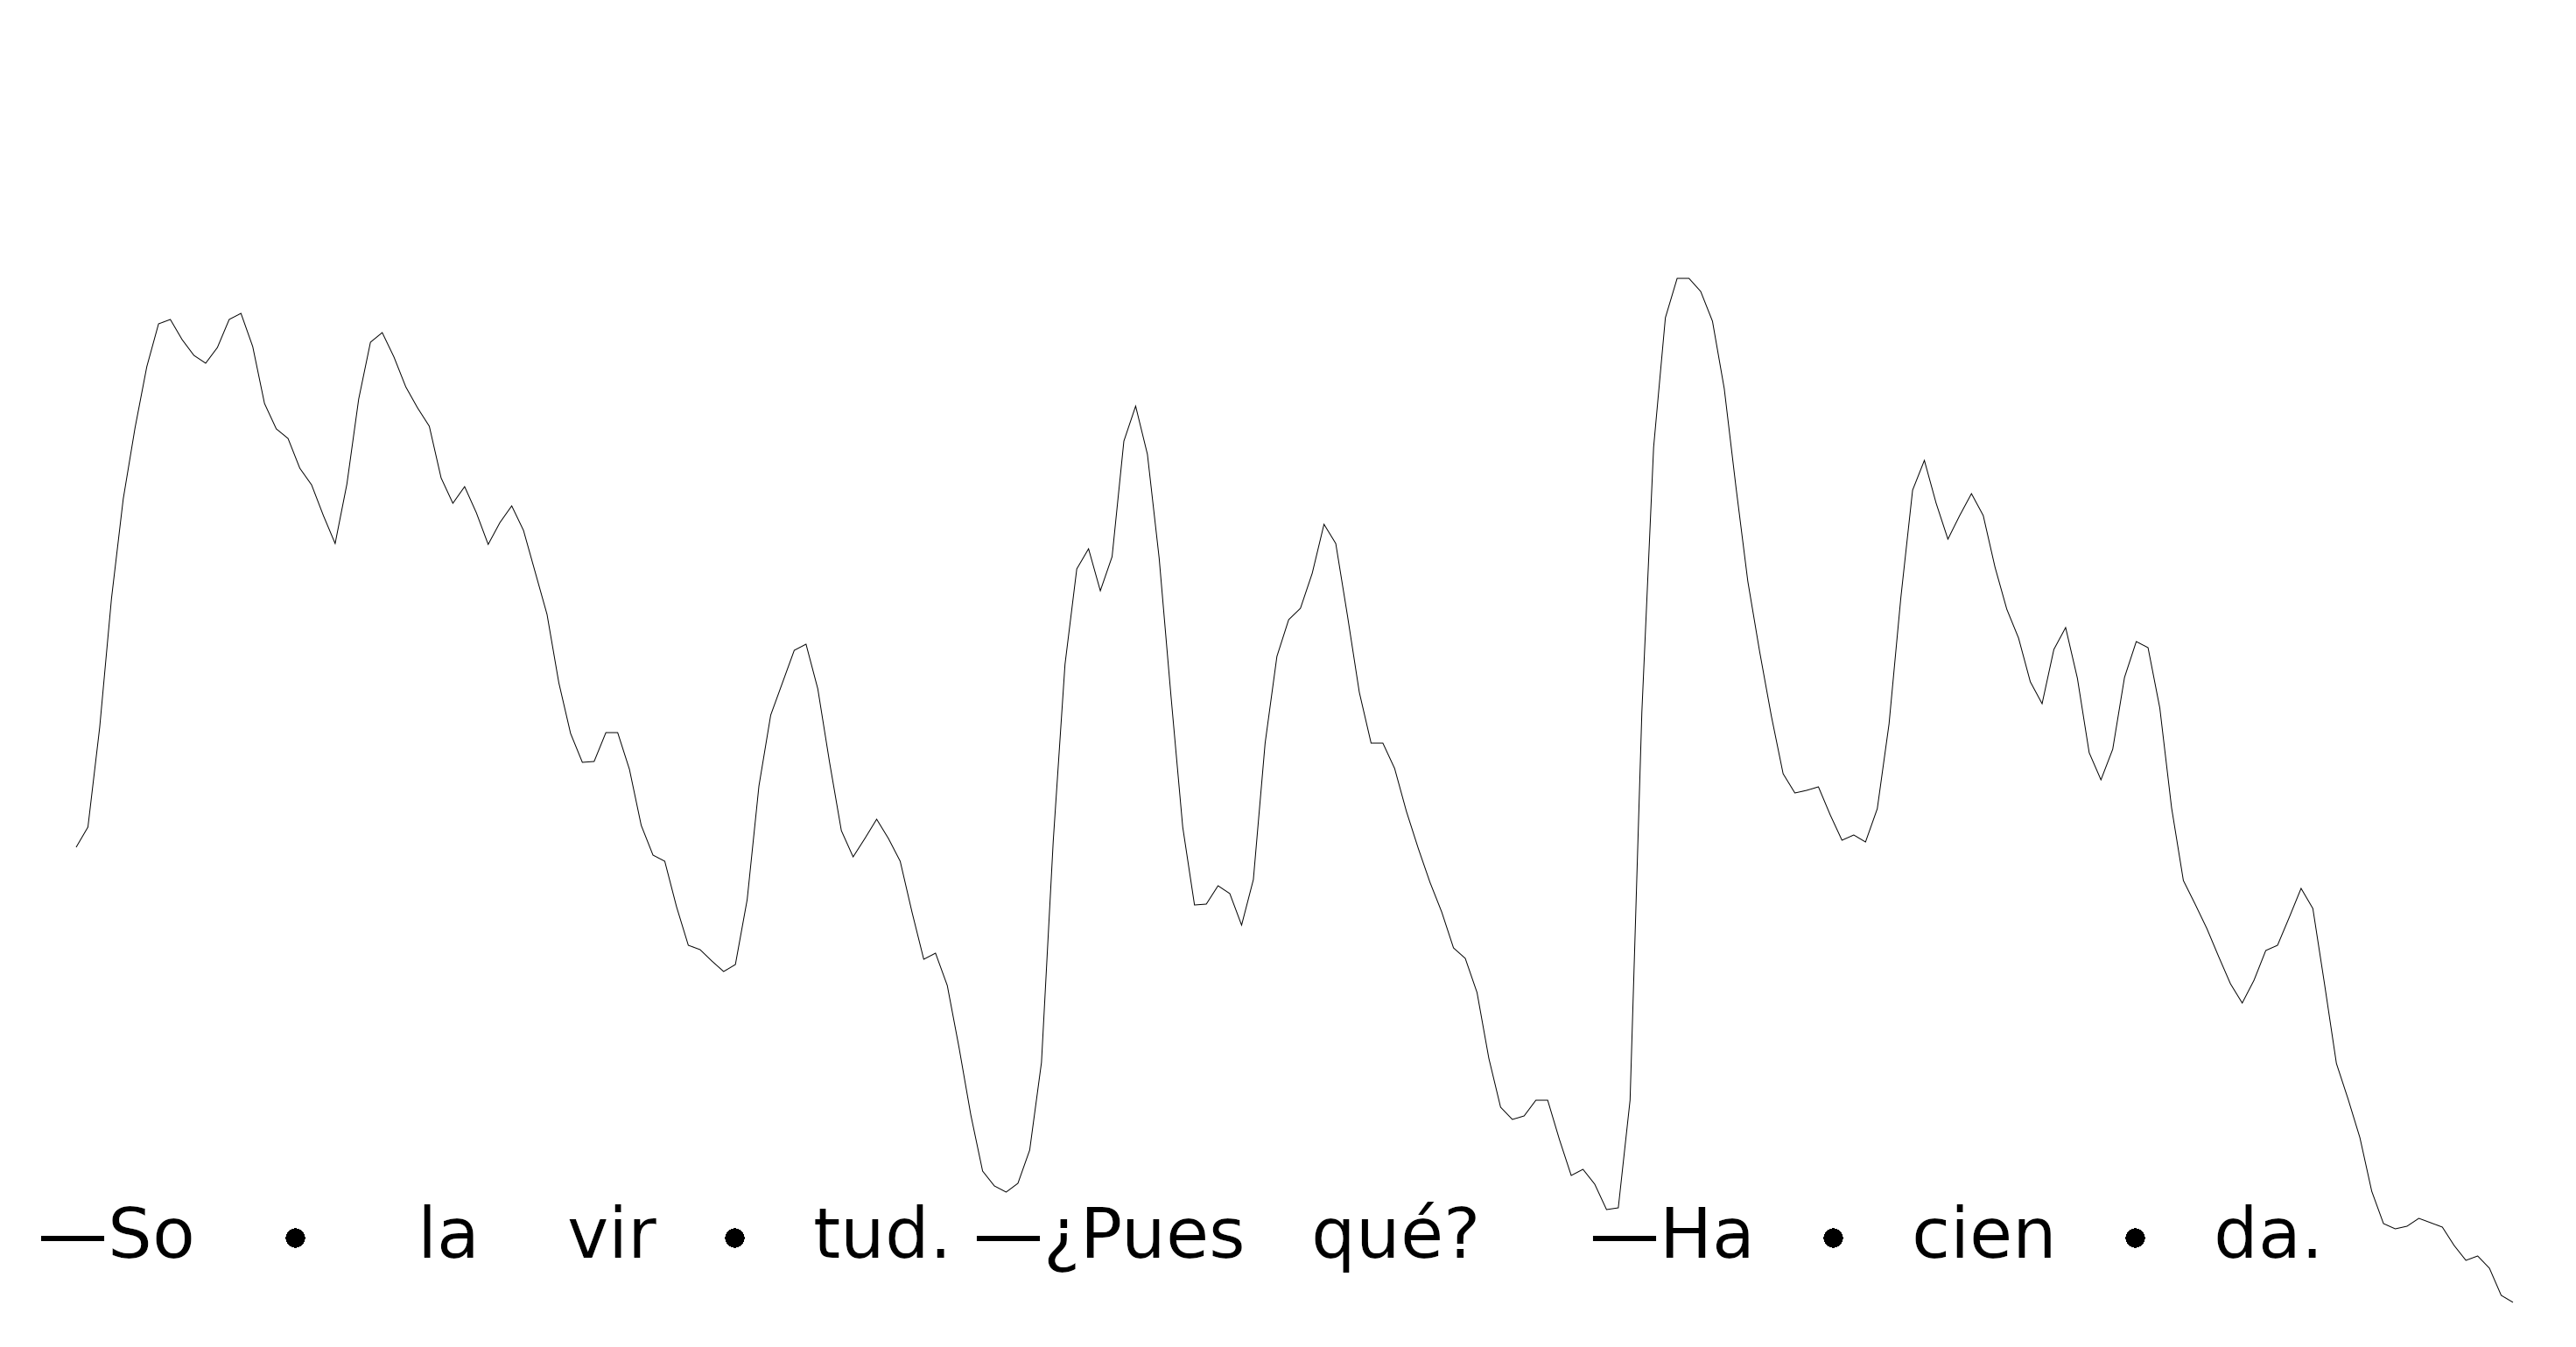
\includegraphics[height = 8cm]{images/solavirtud.png}    
	\caption{Verso 42 en una representación \parencite{vega1982} de \textit{La discreta enamorada}.}
	\label{fig:solavirtud}
\end{figure}

\subsection{Separación de vocales}
Se denomina \textit{diéresis}\index{diéresis} a la ruptura de  una unión natural entre vocales, de forma que el diptongo da lugar a dos sílabas independientes. En lo concerniente a nuestro trabajo, hay que tener en consideración que, a pesar de que estas vienen señaladas explícitamente en las ediciones más minuciosas (por ejemplo, \textlangle{}rüin\textrangle{} /ruˈin/ frente a \textlangle{}ruin\textrangle{} /ˈrwin/), no tiene por qué ser así en todos los casos y, de hecho, no suele serlo. Sin embargo, hay palabras cuyos diptongos se rompen de manera más frecuente en los versos áureos, como \textit{juez}, \textit{suave}, \textit{cruel}, \textit{fiel}, \textit{ruin} y sus derivados, por lo que, si se presenta la necesidad de producir una sílaba adicional para cuadrar el verso, este tipo de palabras se prestan sobremanera a la diéresis. Incluso vates tan poco dados a extravagancias como Quevedo recurren al hiato aprovechándolas, si bien con mucho más comedimiento que sus contemporáneos culteranos \parencite[55-64]{llamas2020}.

Otro fenómeno divisorio es el \textit{hiato}\index{hiato} o la ruptura de una sinalefa. Quilis~\parencite*[50-52]{quilis2013} atribuye el fenómeno a diversas causas, como la acentuación de una de las dos vocales implicadas, causa de sinalefa violenta. En la poesía del Siglo de Oro hay que contemplar asimismo la posible aspiración de la hache inicial en la segunda palabra que, como dijimos, también podría impedir la sinalefa.


\section{Rima}
El medio más evidente de alcanzar eufonía es la rima. Este recurso lírico consiste en la repetición de sonidos desde la última vocal acentuada o cumbre tonal\index{cumbre tonal} del verso. Puede ser de diferentes clases dependiendo de los tipos de sonido que se repitan \parencite[103-115]{dominguez2014a}. No es la única vía para crear un efecto melódico, sino que es frecuente encontrar también otras figuras de repetición tales como aliteración, simetría o anáfora \parencite[126-129]{dominguez2014a}. Podemos definir la rima, pues, como «la total o parcial semejanza acústica, entre dos o más versos, de los fonemas situados a partir de la última vocal acentuada» \parencite[37]{quilis2013}.

De esta manera, hablaremos de rima oxítona\index{rima!oxítona} o \textit{masculina}\index{rima!masculina|see {rima oxítona}} si el verso acaba en palabra aguda\index{palabra!aguda}, paroxítona\index{rima!paroxítona} o \textit{femenina}\index{rima!femenina|see {rima!paroxítona}} si acaba en palabra llana\index{palabra!llana} y proparoxítona\index{rima!proparoxítona} o dactílica\index{rima!dactílica|see {rima proparoxítona}} si acaba en palabra esdrújula\index{palabra!esdrújula}.

Caramuel~\parencite*[57]{caramuel2007} distingue entre rimas \textit{asonantes}\index{rima!asonante}, también llamadas parciales\index{rima!parcial|see {rima asonante}}, cuyas vocales coinciden, pero no así sus sonidos consonánticos (\ref{ex:asonante}), y rimas \textit{consonantes}\index{rima!consonante}, también llamadas rimas totales\index{rima!total|see {rima consonante}}, cuyas vocales y consonantes coinciden desde el último acento (\ref{ex:consonante}). 

\begin{exe}
	\ex\label{ex:asonante}
	\begin{tabular}{l|ll|}
		\cline{2-3}
		Yo, acudiendo a mis es-&t/\textit{ú}-& di/\textit{o}/s\\
		en ellos y en todo &m/\textit{í}-& r/\textit{o}\\
		que Segismundo se- &r/\textit{í}-& \textit{a}\\
		el hombre más atre-&v/\textit{í}-& d/\textit{o},\\\cline{2-3}
	\end{tabular}\\\strut\hfill(Calderón, \textit{La vida es sueño}, vv. 708-711\nocite{calderon_lavidaessuenno})
	\ex\label{ex:consonante}
	\begin{tabular}{l|l|}
		\cline{2-2}
		Hipogrifo vio-&l/\textit{énto},\\
		que corriste parejas con el&vi/\textit{énto}\\\cline{2-2}
	\end{tabular}\\\strut\hfill(vv. 1-2)	
\end{exe}

No todos los sonidos son parte de la rima. En el caso de la rima proparoxítona\index{rima!proparoxítona}, como ya indicamos, la constituyen los elementos de la sílaba tónica y la última sílaba (\ref{ex:proparox}), de manera que \textit{fábula} rima con \textit{águila}. En las rimas asonantes, solo los núcleos vocálicos son relevantes para la rima, de forma que \textit{inercia} rima con \textit{lenta} \parencite[89]{herrero1996}. Aquí es donde se hacen más vez patentes los beneficios de la decisión inicial de partir de una transcripción fonológica silabeada en lugar de la representación ortográfica (\ref{ex:as}). Por una parte, en tanto que tenemos el verso ya separado en sus sílabas, trabajaremos directamente con estas, corrigiendo según los fenómenos intervocálicos si es menester. Por otra parte, al distinguir entre los alófonos vocálicos silábicos y no silábicos, la resolución de la rima asonante es trivial, pues basta con tener en cuenta exclusivamente los fonemas vocálicos silábicos del \textit{axis}\index{axis rítmico} —que discutiremos abajo— de cada verso.

\begin{exe}
	\ex\label{ex:proparox}
	\begin{tabular}{l|l|l|l|}\cline{2-2}\cline{4-4}
	Al Uni-&gé-&ni-&to,\\
	al Padre &m/\textit{á}-&xi-&m/\textit{o}\\
	y al Santo Es-&pí-&ri-&tu,\\
	de ambos Pa-&r/\textit{á}-&cli-&t/\textit{o},\\
	pidamos &hú-&mi-&les,\\
	que en estos &\textit{á}/s-&pe-&r/\textit{o}-/s\\
	valles de &lá-&gri-&mas\\
	desiertos y &\textit{á}-&ri-&d/\textit{o}/s,\\
	su Amor a-&yú-&de-&nos,\\
	su Gracia &s/\textit{á}/l-&ve-&n/\textit{o}/s.\\
	\cline{2-2}\cline{4-4}
\end{tabular}\\
	\strut\hfill(Calderón, \citetitle[855-863]{calderon_annosantoroma})
\ex\label{ex:as}
	\begin{tabular}{l|ll|}\cline{2-3}
Que estas señoras da-&rán,&\\
de irlas sirviendo li-&c/\textit{é}/n-&ci/\textit{a}.\\
Y más cuando fuera& cul-&pa,\\
que los crïados que& d/\textit{é}-&j/\textit{a}/n\\
a sus dueños en vi-&si-&ta,\\
por ellos, Félix, no& vu/\textit{é}l-&v\textit{a}/n.\\
\cline{2-3}
\end{tabular}\\
	\strut\hfill(Calderón, \textit{¿Cuál es mayor perfección...?}, vv. 938-943\nocite{calderon_mayorperfeccion})
\end{exe}

Los versos que acaban con palabras homógrafas suponen un caso particular. Diremos que son \textit{equisonantes}\index{rima!equisonante} si estas difieren léxicamente o en su función gramatical, es decir, si se trata de una diáfora. Lo vemos en el ejemplo \ref{ex:equisonante}, donde \textit{pasa} toma el valor de `entrar' en el segundo de los versos, mientras que vale `acontecer' en el tercero. Si las palabras, además de ser homógrafas, también comparten significado y función, hablamos de rimas \textit{unisonantes}\index{rima!unisonante} (\ref{ex:unisonante}), que resulta inaceptable para la prescriptiva.
\begin{exe}
		\ex\label{ex:equisonante}
		[...]\\
		pero tu hermano viene. Aquí escondida\\
		le he de escuchar. Pues ya a tu cuarto \textit{pasa}.\\
		Y así saber espero lo que \textit{pasa}.\\
		\strut\hfill(Moreto, \textit{No puede ser el guardar una mujer}, vv. [1411-1413\nocite{moreto_nopuedeser})
	\ex\label{ex:unisonante}Colgad ese saco ahí\\
	para que diga, ay de \textit{mí}:\\
	«En tal puesto me colgó\\
	Paulo, que no mereció\\
	la gloria que encierro en \textit{mí}».\\
	\strut\hfill(Tirso de Molina, \citetitle[1885-1889]{tirso_desconfiado})                                         \end{exe}
En cualquier caso, estas restricciones solo afectan a la rima, por lo que, por ejemplo, el primer y segundo verso del ejemplo \ref{ex:norima} no estarían sujetos a estas restricciones y, si bien podría achacársele a Rojas Zorrilla un uso repetitivo del léxico en este caso, esto no tendría repercusión en su observancia de las reglas de la métrica.
\begin{exe}	
\ex\label{ex:norima}En tu atención. El amor,\\
¿quién le colige en lo a\textit{tento}?\\
La atención supone amor,\\
disgusto el diverti\textit{miento};\\
bien quiere aquel que escuchando\\
se transforma en los con\textit{cetos};\\
\strut\hfill(Rojas Zorrilla, \citetitle[31-36]{rojas_obligados})
\end{exe}

Sea como fuere, en el corpus que manejamos, el recurso a la equisonancia se utiliza de manera muy esporádica. La unisonancia es prácticamente inexistente, puesto que esta suele ser fruto de la falta de habilidad del poeta y, si las ediciones digitales de literatos áureos consagrados son escasas, más aún lo son las de los diletantes. La adscripción a uno u otro caso de homofonía de las ocurrencias que hemos encontrado suele ser susceptible de discusión. En cualquier caso, la máquina contaría con los medios para identificar estas rimas, ya que la determinación del ritmo\index{ritmo} obliga a identificar las funciones morfosintácticas de las palabras del verso. Por lo tanto, requeriría apenas verificar que ambos homógrafos de la rima tienen etiquetas diferentes.

Además de la rima externa, aparece aunque no resulta frecuente —Lope se vale de este recurso en, por ejemplo, \textit{El amigo hasta la muerte} y \textit{El mayordomo de la duquesa de Amalfi}— una rima interna italianizante, a imitación del \textit{endecasillabo incatenato}\index{verso!endecasílabo}. Esta rima interna la conforman las del axis rítmico y otro interno que pasa por la sexta sílaba, en el siguiente verso \parencite{sanchez2014}. 

\section{Agrupaciones de versos}
El verso por sí mismo no constituye un elemento lírico. Para que este sea digno de su nombre, debe aparecer en combinación con otros versos \parencite[95]{quilis2013}, de manera que formen una estructura superior que produzca el contexto sonoro de la poesía. Desde el punto de vista semántico, el verso es autosuficiente, pero no así desde el rítmico y sonoro, ya que ha de mostrar un patrón. Como es obvio, para que este pueda existir, se requiere, al menos, una serie de dos elementos. A esta agrupación estructurada de versos la denominamos estrofa\index{estrofa}. A su vez, cabe agrupar varias estrofas en un poema\index{poema!estrófico} estrófico, pero también pueden unirse versos directamente en poemas no estróficos\index{poema!no estrófico}.

\subsection{La estrofa}
De acuerdo con Quilis~\parencite*[95-99]{quilis2013}, la estrofa ha de cumplir cuatro requisitos para ser tal en propiedad: debe tener un \textit{axis rítmico}\index{axis rítmico}\footnote{Emplearemos este cultismo —que Quilis adopta de Balbín~Lucas~\parencite*{balbin1968} —, pues \textit{eje} \index{eje} podría llevar  a confusión, ya que también equivale a la sexta sílaba del endecasílabo\index{verso!endecasílabo} si esta va acentuada \parencite[][\textit{s.v.} \textit{eje}]{dominguez1985}.}, consistir de un número determinado de rimas, poseer una estructura sintáctica determinada y estar dispuesta según un modelo versal estructurado.

El axis rítmico, según como lo define Balbín~\parencite*[38-60]{balbin1968}, está constituido por la inflexión distensiva de cada uno de los grupos melódicos de los que se compone la estrofa en torno a la que se concentran y organizan los factores rítmicos.  Dicho de otra manera, el axis rítmico de la estrofa se establece a partir de la última sílaba acentuada de sus versos (\ref{ex:axis}). Esta es la que carga con el acento versal que, a su vez, altera la cantidad del verso. Aquí se produce asimismo la inflexión del tono; en torno a este punto se distribuyen las pausas para lograr la eufonía y se define el tipo de encabalgamiento.  El centro del eje provee el elemento más importante de la rima. En consecuencia, resulta crucial para nuestro modelo identificar esta parte del verso porque varios de los análisis que han de hacerse se sustentan en su correcta caracterización. Esto significa, además del silabeo, localizar la sílaba que carga con el acento léxico de la última palabra del verso.

\begin{exe}
	\ex\label{ex:axis}
		\begin{tabular}{l|l|l}
			\cline{2-2}
			¿cuál de vosotras, cuál desde su a-&\textit{si/é/n} & -to\\
			es la que influye en mí desdichas&	\textit{t/á}	& -les\\
			¿Cuál de vosotros, astros desi-&	\textit{gu/á}	& -les\\
		a su cargo tomó mi sufri-&				\textit{mi/é/n} & -to\\\cline{2-2}
		\end{tabular}\\
	\strut\hfill(Calderón, \citetitle[653-656]{calderon_suennoshay})
\end{exe}

El número de rimas resulta asimismo fundamental, pues la función de estas no se limita a la ejercida sobre el propio verso, sino que se combinan unas con otras de forma que, de esta unión, resulta una estrofa, cuya configuración es producto del número de rimas y de su distribución. Como veremos un poco más adelante, clasificamos las estrofas en primer lugar por el número de versos que las constituyen y, además, distinguimos entre estrofas con el mismo número de versos por la disposición de las distintas rimas de estos.

Por otra parte, la estrofa encuentra una correspondencia en la estructura sintáctica completa, de manera que la pausa estrófica coincide con el final de la unidad sintáctica. Aunque así se ha hecho tradicionalmente, algunos poetas con querencia por los modelos grecolatinos contravienen la prescriptiva de la métrica castellana para disociar una unidad sintáctica en dos estrofas \parencite[97]{quilis2013}. De la importancia de esta costumbre para reproducir el metro clásico da cuenta el elogio de Menéndez~Pelayo a Francisco Medrano, al que el erudito se refiere como \blockquote{de todos los imitadores de Horacio el más latino, el más sobrio, el más rápido, el que mejor ha remedado la marcha de los períodos rítmicos de Horacio, \textit{el que más se le parece en la manera de encabalgar las estrofas}, y el que más le anda a los alcances en el arte de economizar las palabras. \parencite[p. 14; énfasis añadido]{menendezpelayo1951}}.

En lo que respecta al sistema de estructurar las rimas, cada estrofa debe componerse de un número determinado de versos de tipos concretos dispuestos según un patrón dado. De esta manera, encontramos \textit{estrofas isométricas}\index{estrofa!isométrica}, en las que todos sus versos tienen la misma cantidad, como en el cuarteto del ejemplo \ref{ex:isometrica}, y \textit{estrofas heterométricas}\index{estrofa!heterométrica}, en las que se mezclan versos con distinto número de sílabas (\ref{ex:heterométrica}).

\begin{exe}
	\ex\label{ex:isometrica}Cuando la fama en lenguas dilatada\\	
	vuestra rara hermosura encarecía,\\
	por fe os amaba yo, por fe os tenía,\\ 		
	Leonor, dentro del alma idolatrada.\\
	\strut\hfill(Calderón, \citetitle[746-749]{calderon_secretoagravio})
	\ex\label{ex:heterométrica}Ilustre es, si no rico,\\
	el condado Anspurg en Alemania;\\
	a su quietud me aplico,\\
	pues los jardines de la gran Campania\\
	no igualan a este monte\\
	que el Ártico nos muestra en su horizonte.\\	
	\strut\hfill(Mira de Amescua, \citetitle[89-94]{mira_casaaustria})
\end{exe}
Para representar la estructura de las estrofas, emplearemos, además de la notación tradicional categórica de letras mayúsculas y minúsculas, la de subíndices si la caracterización de la estrofa requiere una descripción cuantitativa de sus versos. De esta manera, representaremos la estrofa del ejemplo \ref{ex:heterométrica} como \textit{aBaBcC} o $a_{7} b_{11} a_{7} b_{11} c_{7} c_{11}$, según las características que convenga observar en cada momento. La segunda forma resulta muy conveniente en una obra dramática, en la que, al contrario de lo que suele ocurrir en los poemas\index{poema}, se alternan diferentes metros, sobre todo de arte menor. De esta manera, resulta más sencillo explorar los versos en su contexto para conocer el uso de una determinada rima y condicionarlo al número de sílabas o viceversa.

Según la disposición de la rima en la estrofa, se distingue entre rima \textit{continua}\index{rima!continua}, con una estructura $aaaa$ (\ref{ex:continua}); \textit{rima gemela}\index{rima!gemela}, según el patrón $aa:bb$ (\ref{ex:gemela}); \textit{rima encadenada}\index{rima!encadenada}, con el patrón $abab$ (\ref{ex:encadenada}) y rima abrazada\index{rima!abrazada}, $abba$ (\ref{ex:abrazada}).

\begin{exe}
	\ex\label{ex:continua}Ay de opinión tan ciega,\\
	que los principios a la Fe le niega,\\
	donde a mover la Caridad no llega,\\
	que huye a Misericordia que le ruega!\\
	\strut\hfill(Calderón, \citetitle[779-982]{calderon_nuevohospicio})
	\ex\label{ex:gemela}Sí, mas de ambiguas razones\\
	en sus ojos mis pasiones\vspace{.333\baselineskip}\\
	han visto lo que me estima.\\
	Vana esperanza te anima\vspace{.333\baselineskip}\\
	cuando penetra mi amor\\
	el que me tiene interior.\vspace{.333\baselineskip}\\
	Cuando tu soberbia abajes\\
	y amor se obligue a mis gajes,\vspace{.333\baselineskip}\\
	tu engaño conocerás.\\
	Yo sé que me envidiarás.\\
	\strut\hfill(Tirso de Molina, \textit{Santo y sastre}, vv. 908-917)\nocite{tirso_santoysastre})
	\ex\label{ex:encadenada} Con el cuidado que el Amor, Diana,\\
	pone en un pecho, que aquel fin desea,\\
	que la mayor dificultad allana,\\
	Él mismo quiere que te adore y vea.\\
	\strut\hfill(Lope de Vega, \citetitle[689-692]{vega_perrohortelano}
	\ex\label{ex:abrazada}Tienes, Laurencia, razón;\\
	que en dejando de querer,\\
	más ingratos suelen ser\\
	que al villano el gorrión.\\ 
	\strut\hfill(\citetitle[249-242]{vega_fuenteovejuna})
\end{exe}


\subsection{Tipología estrófica}
Como indicamos al comienzo de este capítulo, el metro dramático no se diferencia del lírico. Por lo tanto, si hemos de encontrar patrones en las agrupaciones de versos, debemos recurrir a la poética tradicional. Añadiremos que el teatro no solo toma prestada la métrica de la poesía, sino que, además, lo hace extensivamente, aprovechando todos los recursos que aquella pone a su disposición. Así, Fernández Guillermo \parencite*[213-242]{fernandez2021} encuentra en apenas veinte comedias de Lope de Vega —un único autor— las siguientes formas: redondillas, romances con y sin estribillo con hexasílabos\index{verso!hexasílabo} y octosílabos\index{verso!octosílabo}, quintillas, pareados, tercetos sueltos y encadenados, endecasílabos\index{verso!endecasílabo} y otros versos sueltos, octavas, octavas reales, sonetos, canciones, décimas, sextinas, letrillas, coplas, coplillas, seguidillas, seguidillescas, glosas de tipos diversos, silvas, romancillos de ocho y siete sílabas, liras, sextetos-lira, cuartetas asonantadas, canciones petrarquistas, ensaladas, coplas de pie quebrado, villancicos y zéjel, así como partes cantadas con otras medidas y estrofas. A cuenta de esto, resulta necesario caracterizar las agrupaciones versales que encontraremos porque habremos de identificarlas en la segunda parte de este trabajo.

Nos aproximaremos a la clasificación estrófica típica del Siglo de Oro considerando formas recogidas por \citeauthor{morley1968}~\parencite*{morley1968} en su seminal trabajo sobre la datación de la obra lopesca. Optamos por este y no por la obra similar calderoniana de Hilborn~\parencite*{hilborn1938} por encontrarse esta última más simplificada \parencite[3-4]{antonucci2023}. Nos centraremos en las formas españolas \parencite[38-39]{morley1968} e italianas \citedate*[39-41]{morley1968}, como también los metros que constan en las tablas de \citeauthor{fernandez2021}~\parencite*[213-242]{fernandez2021}. Partiremos del número de versos que componen cada estrofa, tomando las descripciones de los tratados de métrica \parencites[102-153]{herrero1996}[100-119]{quilis2013}, e iremos ilustrando sus particularidades con ejemplos del corpus teatral. Esta clasificación será la que tomemos como modelo inicial para reconocer patrones en la segunda parte.

La estrofa más elemental es el \textit{pareado}\index{pareado}, ya que está compuesta de tan solo dos versos de igual o distinto metro y es autosuficiente. Al ser solo dos versos independientes del contexto, solo admiten un patrón de rima en la forma $AA$ (\ref{ex:pareado}). Si, además, los versos son octosílabos\index{verso!octosílabo} con rima consonante $a_{8}a_{8}$, la estrofa se denomina \textit{aleluya}\index{aleluya}. El pareado no ha de ser necesariamente isométrico, sino que también se da entre versos de distinta medida. Un ejemplo paradigmático lo ofrece la combinación de heptasílabos\index{verso!heptasílabo} y endecasílabos\index{verso!endecasílabo} de los pares de versos que componen la \textit{silva de consonantes}\index{silva!de consonante} del monólogo con el que Rosaura da comienzo a \textit{La vida es sueño} (\ref{ex:silvaconsonante}).

\begin{exe}
	\ex\label{ex:pareado}Éste dice: «Señor, yo soy Estacio,\\
		que estoy en los jardines de palacio,\vspace{.333\baselineskip}\\
		y enseñado a plantar hierbas y flores,\\
		planté seis hijos, a los dos mayores\vspace{.333\baselineskip}\\	
		suplico que les deis...».\\
		\strut\hspace{10em}Basta, ya entiendo,\\
		con más cuidado ya premiar pretendo.\\
	\strut\hfill(Lope de Vega, \citetitle[2467-2472]{vega2019})
	\ex \label{ex:silvaconsonante}Hipogrifo violento,\\
	que corriste parejas con el viento,\\
	¿dónde, rayo sin llama,\\
	pájaro sin matiz, pez sin escama,\\
	y bruto sin instinto\\
	natural, al confuso laberinto\\
	de esas desnudas peñas\\
	te desbocas, te arrastras y despeñas?\\
	\strut\hfill(Calderón, \citetitle[1-8]{calderon_lavidaessuenno})
\end{exe}

De cualquier manera, al haber una única rima posible, el nexo entre estrofas del mismo tipo ha de ser débil, en tanto que la siguiente o bien tiene la misma rima, en cuyo caso no hay un cambio, o una diferente, por lo que el salto será abrupto. No es factible una transición entre pareados que además sea suave. Para que esto sea posible, debemos contemplar la estrofa respecto a otras, lo que es el caso del \textit{perqué}\index{perqué} o \textit{aquelindo}\index{aquelindo|see {perqué}}, que alterna rimas que encadena con la siguiente estrofa según la estructura $ab/bc/cd/de...$

\begin{exe}
	\ex\label{ex:perque}\begin{multicols}{2}Escucha, la que veniste\\
	de la jerezana tierra\vspace{.333\baselineskip}\\	
	a hacer a Sevilla guerra\\
	en cueros, como valiente;\vspace{.333\baselineskip}\\	
	la que llama su pariente\\
	al gran Miramamolín;\vspace{.333\baselineskip}\\		
	la que se precia de ruïn,\\
	como otras de generosas;\vspace{.333\baselineskip}\\	
	la que tiene cuatro cosas,\\
	y aun cuatro mil, que son malas;\vspace{.333\baselineskip}\\	
	la que pasea sin alas\\
	los aires en noche escura;\vspace{.333\baselineskip}\\	
	la que tiene a gran ventura\\
	ser amiga de un lacayo;\vspace{.333\baselineskip}\\
	la que tiene un papagayo\\
	que siempre la llama puta;\vspace{.333\baselineskip}\\
	la que en vieja y en astuta\\
	da quinao a Celestina;\vspace{.333\baselineskip}\\
	la que, como golondrina,\\
	muda tierras y sazones;\vspace{.333\baselineskip}\\
	la que a pares, y aun a nones,\\
	ha ganado lo que tiene;\vspace{.333\baselineskip}\\
	la que no se desaviene\\
	por poco que se le dé;\vspace{.333\baselineskip}\\
	la que su palabra y fe\\
	que diese, jamás guardó;\vspace{.333\baselineskip}\\
	la que en darse a sí excedió\\
	a las godeñas más francas;\vspace{.333\baselineskip}\\
	la que echa por cinco blancas\\
	las habas y el cedacillo.\end{multicols}\strut\hfill(Cervantes, \citetitle[556-596]{cervantes1997})
\end{exe}

Del mismo modo, las transiciones entre estrofas se multiplican en el momento en que introducimos un nuevo verso. Las estrofas de tres versos se denominan \textit{tercetos}\index{terceto} en su versión de arte mayor $ABA$ (\ref{ex:terceto}) y tercerillas en las de arte menor\index{tercerilla} $aba$ (\ref{ex:tercerilla}). De esta manera, se dan estrofas $AAA$, que diferirían de los pareados en la cantidad de versos, aunque no en la cualidad de la rima, pero también $ABA$ o $ABB$, que introducirían una alternancia en la rima. Esto, a su vez, expande las posibilidades de combinar estrofas porque ahora podemos encadenarlas en la forma $ABA BCB CDC ...$, de modo que la nueva rima sirve de solución de continuidad para la transición de un verso, pero, al contrario que en la estrofa de dos sílabas, la estrofa puede conservar una rima característica distinta de la siguiente. En la poesía medieval se cultivaba una variante del terceto conocida como \textit{trístico monorrimo}\index{trístico monorrimo}, que tiene la misma rima en sus tres versos según el modelo $AAA$ (\ref{ex:tristico}).
  
 \begin{exe}
 	\ex\label{ex:terceto}Si yo pensara, Conde, que te diera\\
 		tanta tristeza el casamiento mío,\\
 		antes de imaginarlo me muriera.\\
 		\strut\hfill(Lope de Vega, \citetitle[114-116]{vega2019})
 	\ex\label{ex:tercerilla}Si aborrecidas adoran,\\
 	si adoradas aborrecen,\\                                              
 	¡lo que son mujeres!\\	
 	\strut\hfill(Rojas Zorrilla, \textit{Lo que son mujeres}, vv. 2849-2851\nocite{rojas_loquesonmujeres})
 	\ex\label{ex:tristico}Pues los músicos digan a coros:\\
 	No están todos\\
 	en la casa de los locos.\\	
 	\strut\hfill(vv. 2701-2703)
 	\end{exe}
 	
 	
Las estrofas de cuatro versos ofrecen más variedad. Si son consonantes de arte mayor, se denominan \textit{cuartetos}\index{cuarteto}, y tienen rima cruzada $ABBA$ o encadenada $ABAB$ (\ref{ex:cuarteto}), en cuyo caso reciben el nombre de \textit{serventesio}\index{serventesio}. En cuanto a las de arte menor, tenemos la \textit{cuarteta}\index{cuarteta} según el esquema $abab$ (\ref{ex:cuarteta}). La combinación de arte menor se conoce como \textit{redondilla}\footnote{No confundir con la \textit{redondilla} según la terminología de Díaz~Rengifo~\parencite*[193-207]{diazrengifo2012}, quien emplea el término para referirse a estrofas de octosílabos\index{verso!octosílabo} de cinco versos y sus variaciones de entre cuatro y ocho.}\index{redondilla} si la rima es abrazada en la forma $abba$ (\ref{ex:redondilla}). Una variante de esta estrofa es aquella que solo rima en sus versos pares según el modelo $-a-a$. Se da también la modalidad \textit{asonantada}\index{cuarteta!asonantada} o \textit{tirana}\index{cuarteta!tirana|see {cuarteta asonantada}} (\ref{ex:asonantada}). La redondilla en secuencia con el romance es la estrofa más común en el teatro de Lope \parencite[169]{fernandez2007}, cuya obra representa un porcentaje notable de la producción dramática del Siglo de Oro que ha llegado hasta nosotros. 

\begin{exe}
	\ex\label{ex:cuarteto}Amor de ser amado satisfecho\\
	cuando agraviado imaginó vengarse,\\
	Templado el fuego y el furor desecho,\\
	Adonde pudo arderse pudo helarse.\\
	\strut\hfill(Lope de Vega, \citetitle[403]{vega_dorotea})
	\ex\label{ex:cuarteta}Razón, fortuna, amor, celos\\
	son pasiones que se mudan:\\
	la razón falta a su tiempo\\
	y se cansa la fortuna;\\
	\strut\hfill(Calderón, \citetitle[2068-2071]{calderon_bandaflor})
	\ex\label{ex:redondilla}Yo os juro que, si os agrado,\\
	que de vos lo voy también,\\
	y que, procediendo bien,\\
	os doy amor por cuidado.\\
	\strut\hfill(Lope de Vega, \citetitle[65-68]{vega_villano})
	\ex\label{ex:asonantada}Inventó el amor un juego\\
	donde en gustosos descuidos,\\
	pagando en prendas sus yerros,\\
	se vino a quedar desnudo.\\
	\strut\hfill(Moreto, \textit{El hijo pródigo}, vv. 1309-1312\nocite{moreto_hijoprodigo})
\end{exe}

Las estrofas de cuatro versos se prestan bien a diversas combinaciones heterométricas. Así, la \textit{seguidilla}\index{seguidilla} combina versos impares heptasílabos\index{verso!heptasílabo} y pares pentasílabos en su variedad habitual (\ref{ex:seguidilla})\footnote{No confundir con la llamada \textit{seguidilla gitana}\index{seguidilla!gitana}, compuesta de versos hexasílabos\index{verso!hexasílabo} a excepción del tercero que es decasílabo o endecasílabo\index{verso!endecasílabo}, que sería una variante de la endecha \parencite[185-186]{hanssen1957}.}. Navarro Tomás\parencite*[292-293]{navarrotomas1991} recoge variaciones con hexasílabos en lugar de pentasílabos, así como de tres versos, que se reparten según las disposiciones $5-7-5$ y $7-5-7$, y \citeauthor{morley1968}~\parencite*{morley1968} con siete versos $XaYa:bZb$. Asimismo, Sor Juana Inés, entre otras modalidades, usó una conocida como \textit{seguidilla real}\index{seguidilla!real}, según el patrón $x{10}a_6x_{10}a_6$. También heterométrica es la \textit{estrofa sáfica}\index{estrofa!sáfica} (\ref{ex:estrofasafica}), que se compone de tres endecasílabos sáficos  (\texttt{---+x+xxx+-}) y un pentasílabo adónico (\texttt{+xx+x}) o, en su adaptación a la rítmica castellana, un hexasílabo según el patrón \texttt{+x+x+-} \parencite[119]{luque2010}. En la poética castellana, gozaba de gran tradición el \textit{tetrástrofo monorrimo}\index{tetrástrofo monorrimo|see {cuaderna vía}}, más conocido por \textit{cuaderna vía}\index{cuaderna vía}, que se compone de cuatro versos alejandrinos\index{alejandrino}, a su vez formados por dos hemistiquios\index{hemistiquio} heptasílabos cada uno, y una sola rima consonante, pero su presencia es escasa en el Siglo de Oro \parencite[277]{navarrotomas1991}. Entre las formas heterométricas destacan las que constituyen la composición conocida como \textit{endecha real}\index{endecha!real}  (\ref{ex:endechareal}). Si la \textit{endecha}\index{endecha} es un romancillo de versos de menos de ocho sílabas de tema triste \parencite[\textit{s.v.} \textit{endecha}]{dominguez1985}, la real presenta la particularidad de que sus tres primeros versos son heptasílabos y el cuarto endecasílabo.

\begin{exe}
	\ex\label{ex:seguidilla}Alegría, zagales,\\                                                                  
	que a casa vuelve\\
	hoy el hijo perdido.\\
	Todos se alegren.\\
	\strut\hfill(Moreto, \textit{El hijo pródigo}, vv. 2843-2856\nocite{moreto_hijoprodigo})
	\ex\label{ex:estrofasafica}\metrics{u | _ u u | _ u || u _ u u _ u ||}{{A-} | mor po-{de-} | ro-so || en cie-lo \bow{y e}n tie-rra, ||}\\	
\metrics{u | _ u u | _ u || u _ u u _ u ||}{{dul-} | cí-si-ma | gue-rra || de nues-tros sen-ti-dos, ||}\\
\metrics{u | _ u u | _ u || u _ u u _ u ||}{¡oh, | cuán-tos {per-} | di-dos || con vi-d\bow{a i}n-quï-e-ta ||}\\
\metrics{u | _ u u | _ u ||}{{t\bow{u i}m-} | pe-rio {su-} | je-ta! ||}\\
	\strut\hfill(Lope de Vega, \citetitle[158]{vega_dorotea})
	\ex\label{ex:endechareal}No con más diligencia\\
	la diosa de las mieses\\
	buscó a su hija amada\\
	hasta los escondrijos del infierno,\\
	\strut\hfill(Cervantes, \citetitle[515-518]{cervantes_entretenida})
\end{exe}

Hay que hacer notar una característica del ejemplo \ref{ex:estrofasafica} que será conveniente considerar para diseñar el sistema de escansión. Si atendemos a la prosodia, la estrofa está compuesta de tres versos de doce  sílabas y uno de seis. Sin embargo, dijimos que este tipo de estrofa se compone de endecasílabos\index{verso!endecasílabo} y un pentasílabo. Vemos en la correspondencia con los pies del modelo latino del pentasílabo y los primeros hemistiquios\index{hemistiquio} de los endecasílabos que tenemos una sílaba suelta antes del dáctilo y el troqueo. En efecto, está sílaba está en anacrusa, por lo que no se considera en el cómputo silábico ni en el patrón acentual —de cantidad en el modelo latino—. De esta manera,  los acentos de los endecasílabos recaen en la primera y cuarta sílaba tras la anacrúsica y en la primera y tercera en el pentasílabo. Dada la escasa frecuencia con que aparecen metros inusuales, cabe plantearse considerar este fenómeno ante versos de metro inesperado con sílabas átonas a comienzo del verso. Por otra parte, el último endecasílabo presenta otra particularidad, ya que requiere contemplar la interjección como inacentuada.

Entre las estrofas isométricas de cinco versos, el \textit{quinteto}\index{quinteto}, de arte mayor, no es habitual en la poesía aurisecular, al contrario que su equivalente de arte menor, la \textit{quintilla}\index{quintilla} (\ref{ex:quintilla}). Ambas formas presentan restricciones, pues han de tener rima consonante, no contienen más de dos versos seguidos con la misma rima, los dos últimos versos no riman entre sí y no hay versos sueltos, de manera que solo se dan las combinaciones $ABABA$, $ABAAB$, $ABBAB$, $AABAB$ y $AABBA$. Entre las estrofas heterométricas cabe destacar la \textit{lira}\index{lira}, que combina dos endecasílabos\index{verso!endecasílabo} y tres heptasílabos\index{verso!heptasílabo} según la estructura rimante $aBabB$. Aunque apenas encuentra uso dramático tras Rey de Artieda y Juan de la Cueva \parencite[257]{navarrotomas1991}, da pie a otros metros más extendidos como el sexteto-lira.

 \begin{exe}
	\ex\label{ex:quintilla}Y así, en lirio transformado,\\
	siendo el morado color\\
	jeroglífico del prado,\\
	se vio entre el lirio y la flor\\
	el amor enamorado.\\	
	\strut\hfill(Calderón, \textit{Hado y divisa...}, vv. 1604-1608\nocite{calderon_hadoydivisa})
	\ex\label{ex:lira}¿Es, ingrata Sigura,\\
	el casamiento próspero que aguardo?\\
	Callar será cordura,\\
	pues de ira y desdén ardo,\\
	y de envidia me hielo y acobardo.\\
	\strut\hfill(Rey de Artieda, \citetitle[533-537]{reydeartieda_amantes})
\end{exe}

Las estrofas isométricas de seis versos más destacadas son la \textit{sextilla}\index{sextilla} (\ref{ex:sextilla}), con restricciones semejantes a las de la quintilla en cuanto a la disposición de las rimas, así como su equivalente de arte mayor, el \textit{sexteto}\index{sexteto}. La \textit{sextina real}\index{sextina!real} o \textit{sexta rima}\index{sexta rima|see {sextina real}} es una configuración italianizante de versos endecasílabos\index{verso!endecasílabo} según el patrón $ABABCC$, «como una octava real a la que hubiesen recortado los dos primeros versos» \parencite[276]{baehr1997}. Presenta a veces algunas variaciones, como el empleo de versos oxítonos\index{rima!oxítona} en los versos tercero y sexto; no obstante, gozó de escasa estima entre los dramaturgos áureos \parencite[256]{navarrotomas1991}.

\begin{table}[!ht]
	\centering\small
	\begin{tabular}{rlcc}
		\toprule
		Versos&Estrofa&Rima&Distribución\\
		\midrule
		\multirow{4}{*}2&Pareado&indiferente& $a_{x}a_{x}$\\
		&Aleluya&indiferente&$a_{8}a_{8}$\\
		&Perqué&indiferente&$a_{8}b_{8}/b_{8}c_{8}/...$\\
		&Silva de consonantes.&consonante&$a_{7}a_{11}$\\
		\midrule
		\multirow{4}{*}3&Tercerilla&consonante&$aba$\\
		&Terceto&consonante&$a_{11}b_{11}a_{11}$\\
		&Trísticos&indiferente&$a_{x}a_{x}a_{x}$\\\midrule
		\multirow{9}{*}4&Cuarteta&consonante&$abab$\\
		&Redondilla&consonante&$abba$\\   
		&Serventesio&consonante&$ABAB$\\
		&Cuarteto&consonante&$ABBA$\\
		&Copla&asonante&$xaxa$\\
		&Seguidilla&indiferente&$x_{7}a_{5}x_{7}a_{5}$\\
		&Cuaderna vía&consonante&$x_{14}x_{14}x_{14}x_{14}{}^{*}$\\
		&Estrofa sáfica&indiferente&$x_{11}x_{11}x_{11}x_{5}$\\\midrule
		\multirow{3}{*}5&Quintilla&indiferente&$abbab{}^{\dag}$\\
		&Quinteto&consonante&$ABBAB{}^{\dag}$\\
		&Lira&indiferente&$a_{7}b_{11}a_{7}b_{7}b_{11}$\\\midrule
		\multirow{6}{*}6&Sextilla&consonante&$abaaba{}^{\dag}$\\
		&Sexteto&consonante&$ABAABA{}^{\dag}$\\
		&Sexteto correlativo&consonante&$a_{7}b_{7}c_{11}/a_{7}b_{7}c_{11}$\\
		&sexteto-lira&consonante&$a_{7}b_{11}a_{7}b_{11}c_{7}c_{11}$\\
                &Sexta rima&consonante&$a_{11}b_{11}a_{11}b_{11}c_{11}c_{11} / a_{11}c_{11}c_{11}^{\prime}b_{11}b_{11}c_{11}^{\prime}$\\
                &Estrofa manriqueña&consonante&$a_{8}b_{8}c_{4}a_{8}b_{8}c_{4}$\\\midrule
		\multirow{2}{*}7&Séptima&indiferente&$abbab$\\
                &Seguidilla compuesta&indiferente&$x_{7}a_{5}x_{7}a_{5}\:b_{7}a_{5}x_{7}b_{5}$\\\midrule
		\multirow{5}{*}8&Octavilla&consonante&$a_{8}b_{8}b_{8}c_{8}^{\prime}\:d_{8}e_{8}e_{8}c_{8}^{\prime}$\\
		&Octava real&consonante&$a_{11}b_{11}a_{11}b_{11}a_{11}b_{11}c_{11}c_{11}$\\
                &Copla castellana&consonante&$a_{8}b_{8}b_{8}a_{8}\:c_{8}d_{8}d_{8}c_{8}$\\
		&Copla de arte mayor&consonante&$a_{12}b_{12}b_{12}a_{12}\:a_{12}c_{12}c_{12}a_{12}$\\
		&Octava italiana&consonante&$ABBE^{\prime}\: CDDE^{\prime}$\\\midrule
		\multirow{3}{*}{10}&Décima&consonante&$abba\:ac\:cddc$\\
		&Copla real&consonante&$abbab\:cdcdc$\\
                &Ovillejo&consonante&$a_{8}a_{4}b_{8}b_{4}c_{8}c_{4}\:c_{8}d_{8}d_{8}c_{8}$\\
		\bottomrule
		\multicolumn{4}{l}{\footnotesize\textsuperscript{*} También de dieciséis sílabas.}\\
		\multicolumn{4}{l}{\footnotesize${}^{\dag}$ Las rimas alternas de acuerdo a las restricciones descritas.}\\
	\end{tabular}
	\caption{Estrofas.}
	\label{tab:estrofas}
\end{table}


Encontramos asimismo estrofas\index{estrofa!heterométrica} heterométricas, como el sexteto-lira\index{sexteto-lira}, compuesto de heptasílabos\index{verso!heptasílabo} y endecasílabos\index{verso!endecasílabo} en versos alternos, tal como en $aBaBcC$ o $abCabC$ (\ref{ex:sextetolira}). Existen también combinaciones heterométricas de arte menor, como la sextilla\index{sextilla! de pie quebrado} \textit{de pie quebrado}\footnote{También aparece como \textit{copla de pie quebrado}\index{copla!de pie quebrado|see {sextilla de pie quebrado}} (\ref{ex:coplapiequebrado}). Sin embargo, dado que la copla tiene un tamaño variable, optaremos por denominar este metro como sextilla en lugar de utilizar el \textit{hiperónimo} copla.}. Un caso particular de esta estrofa con gran tradición en las letras castellanas es la llamada \textit{estrofa manriqueña}\index{estrofa!manriqueña}, por haberla usado Jorge Manrique en el siglo \textsc{xv} para componer las \textit{Coplas a la muerte de su padre}. En esta estrofa, los tetrasílabos se disponen en el tercer y sexto verso, tal que resulta $a_{8}b_{8}c_{4}a_{8}b_{8}c_{4}$. También de seis versos son las \textit{estrofas aliradas}\index{estrofa!alirada}, que alternan endecasílabos y heptasílabos según el esquema $aBaBcC$ (\ref{ex:estrofalirada}), pero que admiten además otras combinaciones.

\begin{exe}
	\ex\label{ex:sextilla}Si lo que la Infanta yerra\\
	peregrino huésped, curas,\\
	haciendo al infierno guerra,\\
	dirán todas las criaturas:\\
	«¡Gloria a Dios en las alturas,\\
	y paz al hombre en la tierra!».\\
	\strut\hfill(Calderón, \citetitle[1328-1334]{calderon_venenotriaca})
	\ex\label{ex:sextetolira}Aneguen mis enojos\\
	estos campos con llanto de mis ojos.\\
		Y este monte, que ha sido\\
		áspero monumento,\\
		aumente el sentimiento,\\
		aun sin tener sentido,\\
		y, enternecido, el suelo\\
		muestre en su llanto eterno desconsuelo,\\
	\strut\hfill(Calderón, \textit{Judas Macabeo}, vv. 492-497\nocite{calderon_judasmacabeo})
	\ex\label{ex:coplapiequebrado} ¡Qué ventura\\
	que solo el tiempo os destroce,\\
	cuando el sol solo os conoce;\\
	y en esta selva segura,\\
	lo que vuestra vida dura,\\
	libres siempre, nadie os goce!\\	
	\strut\hfill(Calderón, \citetitle[299-304]{calderon_secretoagravio})
	\ex\label{ex:estrofalirada}Un sabio que escribía\\
	en su cama, una vez incorporado,\\
		la mano que movía,\\
		por ser entonces el invierno helado,\\
		de suerte se le helaba\\
		que apenas letra ni razón formaba.\\
	\strut\hfill(Lope de Vega, \textit{Poder vencido y amor premiado}, vv. 3033-3038\nocite{vega_podervencido})
\end{exe}

Las estrofas\index{estrofa} de siete versos no resultan tan productivas en las letras castellanas como las otras que hemos visto. Mencionaremos la \textit{seguidilla compuesta}\index{seguidilla!compuesta} entre las estrofas de este número de sílabas, que se compone de una seguidilla simple y un bordón o estribillo de tres versos adicionales, distribuidos según la forma $x_{7}a_{5}x_{7}a_{5}/b_{5}x_{7}b_{5}$. No obstante, la estrofa varía en sus versos según el bordón. Asimismo, encontramos una extensión a siete versos de la estrofa alirada repitiendo el metro en los dos últimos (\ref{ex:entretenida}).
\begin{exe}
	\ex\label{ex:entretenida}Amor, que lo imposible facilitas\\	
	con poderosa fuerza blandamente,\\
	allanando las cumbres:\\
	¿por qué las nubes de mi sol no quitas?\\
	¿Por qué no muestras por algún Oriente\\	
	las dos hermosas cumbres\\
	que dan rayos al sol, luz a tus ojos,\\
	por quien te rinde el mundo sus despojos?\\
	\strut\hfill(Cervantes, \citetitle[577-584]{cervantes_entretenida})
\end{exe}

Las estrofas de ocho versos gozan de mayor estima en la literatura española. La agrupación isométrica de arte mayor más típica es la \textit{octava}, pero existen diferentes variantes de esta. Así, se conocen estrofas como la \textit{copla de arte mayor}\index{copla!de arte mayor} —también llamada de Juan de Mena, por haberla cultivado este poeta con gran acierto—, que adopta el patrón $a_{12}b_{12}b_{12}a_{12}:a_{12}c_{12}c_{12}a_{12}$. Sin embargo, es muy difícil de encontrar en el teatro del Siglo de Oro. La configuración típica de la copla de arte menor es $abba:acca$ \parencite[266]{navarrotomas1991}. La \textit{octava real}\index{octava real} surge como una modificación de la octava real siciliana, en la que se altera la última rima para obtener un pareado en acorde a $ABABABCC$ (\ref{ex:octavareal}), y se emplea en el teatro para parlamentos graves \parencites[252]{diazrengifo2012}[255]{navarrotomas1991}.

\begin{table}[!ht]
	\centering\small
	\begin{tabular}{llll}
		\toprule
		Enfático&puro&&1-6-10\\
		Enfático&pleno&&1-6-8-10\\
		Heroico&puro&&2-6-10\\
		Heroico&pleno&&2-4-6-8-10\\
		Heroico&corto&&2-4-6-10\\
		Heroico&largo&&2-6-8-10\\
		Heroico&difuso&&2-4-10\\
		Melódico&puro&&3-6-10\\
		Melódico&pleno&&1-3-6-8-10\\
		Melódico&largo&&3-6-8-10\\
		Melódico&corto&&1-3-6-10\\
		Sáfico&puro&&4-8-10\\
		Sáfico&puro&pleno&1-4-8-10\\
		Sáfico&pleno&&1-4-6-8-10\\
		Sáfico&corto&&4-6-10\\
		Sáfico&corto&pleno&1-4-6-10\\
		Sáfico&largo&&4-6-8-10\\
		Sáfico&largo&pleno&2-4-8-10\\
		Sáfico&difuso&&4-10\\
		Sáfico&difuso&pleno&1-4-10\\
		Sáfico&inverso&&1-6-7-10\\
		Vacío&puro&&6-10\\
		Vacío&largo&&6-8-10\\
		Dactílico&puro&&4-7-10\\
		Dactílico&pleno&&1-4-7-10\\
		Dactílico&corto&&2-4-7-10\\
		Galaico&antiguo&&5-10\\
		Italiano&puro&&7-10\\
		\bottomrule
	\end{tabular}
	\caption{Clasificación del endecasílabo.}
	\label{tab:endecasilabos}
\end{table}



En cuanto a las estrofas\index{estrofa!de arte menor} de arte menor, desde el Renacimiento se encuentran \textit{octavillas}\index{octavilla}, pero estas no son más que la unión de dos redondillas en las que una de sus rimas es coincidente. Para el periodo que nos ocupa, entendemos la estrofa como una composición de otras menores, ya que no adquiere entidad propia hasta entrado el siglo \textsc{xviii}, cuando se introduce la \textit{octavilla italiana}\index{cuarteta italiana}, que aporta el rasgo distintivo del último verso agudo de cada semiestrofa. La \textit{copla castellana}\index{copla!castellana} no difiere en esto, aunque sí en la rima de la segunda semiestrofa, de manera que presenta un patrón de según el modelo $abba:cddc$  (\ref{ex:coplacastellana}). Esta forma tuvo cierto predicamento hasta la época de Juan de la Cueva, pero las siguientes generaciones optaron por la redondilla emancipada \parencite[267]{navarrotomas1991}. Pueden ser también de \textit{de pie quebrado} si alternan versos de ocho y cuatro sílabas.

\begin{exe}
	\ex\label{ex:octavareal}«Señor, mirad por vuestra casa atento;\\
	que el Conde y la Duquesa en vuestra ausencia...»\\
	No me ha sido traidor el pensamiento,\\
	habrán regido mal, tendré paciencia.\\
	«ofenden con infame atrevimiento\\
	vuestra cama y honor», ¿Qué resistencia\\
	haran a tal desdicha mis enojos?\\
	«Si sois discretom os lo diran los ojos».\\
	\strut\hfill(Lope de Vega, \citetitle[2484-2491]{vega2019})
	\end{exe}

Las últimas estrofas\index{estrofa} que repasaremos en este capítulo son las compuestas de diez versos. No iremos más allá, puesto que estamos de lleno en el terreno en el que las agrupaciones se consideran estructuras complejas a partir de la combinación de estrofas simples. Sirva para ilutrarlo la copla castellana del ejemplo \ref{ex:coplacastellana}, que podría dividirse en dos estrofas simples, redondillas en este caso. De esta manera, una vez hayamos establecido en la parte práctica el modo de agrupar las estrofas simples, podremos extrapolar el método a cualquier otra forma compleja para clasificarla según patrones estróficos, análogamente a lo hecho con los versos.

\begin{exe}
	\ex\label{ex:coplacastellana}A Dios pongo por testigo,\\
	si a tal quisiera venir,\\
	mas puédeseme decir:\\
	«mensajero sois, amigo».\\
	Que bien saneado estó\\
	que dirán de mi llegada:\\
	«aunque traéis la embajada,\\
	no merecéis culpa, no»\footnote{Nótese que se emplea este metro tradicional para tratar un tema clásico del romancero. No resulta probable que esto sea producto de la mera casualidad, sino que, más bien, sugiere una percepción de la copla castellana como una estrofa arcaizante, lo que bien podría explicar el desuso en el que cayó con la llegada de la Edad Moderna.}.\\	
	\strut\hfill(Juan de la Cueva, \textit{La muerte del rey don Sancho...}, vv. 172-178\nocite{mena_muertereysancho})
\end{exe}

 Así, entre las estrofas de diez versos citaremos la \textit{copla real}\index{copla!real}, que podría analizarse en realidad como la unión de dos quintillas; la \textit{décima}\index{décima} o \textit{espinela}\index{espinela|see {décima}} —ya que se atribuye su invención al ingenio de  Vicente Espinel—, que, a su vez, está compuesta de dos redondillas unidas por dos versos de enlace en los que se repite la primera rima de cada una de las redondillas (\ref{ex:decima}) y, por último, el \textit{ovillejo}\index{ovillejo} o \textit{séptima real}\index{séptima real|see {ovillejo}}, una forma compuesta de tres pareados\index{pareado} octosilábicos y tetrasilábicos y una redondilla\index{redondilla} octosilábica (\ref{ex:ovillejo}).
 
 Existen no obstante construcciones estróficas de verso variable, como la \textit{estancia}\index{estancia}, que combina entre nueve y veinte versos heptasílabos\index{verso!heptasílabo} y endecasílabos\index{verso!endecasílabo} con rima consonante. En su modalidad más regular, consta de una \textit{fronte}\index{fronte@\textit{fronte}|see {frente}} o \textit{frente}\index{frente} y una \textit{sirma}\index{sirma@\textit{sirma}|see {coda (metro)}} o \textit{coda}\index{coda (metro)}. La frente la componen dos \textit{piedi}\index{piede@\textit{piede}|see {pie (metro)}} o \textit{pies}\index{pie (metro)} de tres versos e igual esquema rítmico, denominado el primero \textit{vuelta} o \textit{tornata} y el segundo \textit{revuelta}. La coda comienza con un \textit{eslabón}  (también \textit{chiave}\index{chiave@\textit{chiave}|see {eslabón}}) heptasílabo que rima con el último verso de la fronte, al que siguen otros versos hasta concluir con una coda de pareados. 

\begin{exe}
	\ex\label{ex:decima}\begin{multicols}{2}
	Dorotea: litigantes\\
	sobre tu amor, Lelio y yo,\\
	la esperanza nos citó\\
	a tus estrados amantes.\vspace{.333\baselineskip}\\
	
	Amigos éramos antes;\\
	mas pleitos de tu beldad\vspace{.333\baselineskip}\\	
	mudan nuestra voluntad\\
	en competencia enemiga,\\
	que si es cuerdo, no hay quien diga\\
	que en pleitos hay amistad.\end{multicols}
	\strut\hfill(Tirso de Molina, \textit{Santo y sastre}, vv. 847-856\nocite{tirso_santoysastre})
	\ex\strut\label{ex:ovillejo}\begin{multicols}{2}
		Céfiro, ¿en quién dicha espera?\\
		En una fiera.\vspace{.333\baselineskip}\\
		¿Y quién a Ifis da desmayo?\\
		Un bello rayo.\vspace{.333\baselineskip}\\
		¿En quién Pigmaleón no medra?\\
		En una piedra.\vspace{.333\baselineskip}\\
		\vspace{.333\baselineskip}\\
		Ninguno llegue a ser yedra\\
		del laurel que ama, porque hoy\\
		lloren todos, que yo soy\\
		la fiera, el rayo y la piedra.\\
	\end{multicols}	
	\strut\hfill(Calderón, \citetitle[2060-2069]{calderon_fierarayopiedra})
\end{exe}


\subsection{Poemas estróficos}
Denominamos poemas\index{poema!estrófico} estróficos a aquellos que, como su propio nombre sugiere, están compuestos por estrofas. Esto es, los versos se agrupan en unidades intermedias dentro del poema. En la literatura española se han usado con más o menos profusión diferentes formas, pero los siguientes ocupan un lugar destacado \parencite[126-150]{quilis2013}.

La \textit{canción}\index{canción} es un tipo de poema\index{poema} que proporciona gran libertad compositiva al poeta, ya que, además de no exigirle fijar un número de estrofas concreto, estas también varían en su número de versos. En general, las estrofas\index{estrofa} oscilan entre seis y doce versos en la canción provenzal o nueve y veinte en la petrarquista, así como quince en el modelo de Boscán o trece el de Garcilaso. Tampoco hay una regla fija que dicte la naturaleza de la rima y su distribución. A pesar de todo, hay una estructura global fija, ya que la disposición de la primera estrofa se repite en las siguientes. Cada una de estas estrofas tiene dos partes, unos versos iniciales de frente, que se divide a su vez, por lo general, en dos pies, y una parte final o coda, compuesta por uno más versos o uno o más \textit{volte}\index{volta@\textit{volta}}\footnote{Tomaremos prestado el término de la nomenclatura italiana porque la forma \textit{verso} podría inducir a confusión con uso más común en la métrica.} a imagen de los pies de la frente. La canción concluye con una estrofa más corta, la \textit{tornata}\index{tornata@\textit{tornata}|see {envío}} o \textit{envío}\index{envío}. Puede darse asimismo un eslabón de unión entre frente y coda. Su presencia en el teatro es escasa, aunque no del todo desconocida. En el ejemplo \ref{ex:cancion}, frente y coda tienen dos partes de cuatro versos, el envío también de cuatro y sin verso de enlace.

\begin{exe}
	\ex\label{ex:cancion}\begin{multicols}{2}Llorente pidió a su prima\\
	Constanza le dé a beber,\\
	y ella quísolo hacer\\
	y echóle el cántaro encima.\vspace{.333\baselineskip}\\
	Sintiéndose fatigado\\
	de sed, de amor y calor,\\
	le demandó por favor\\
	agua, estando ya abrasado.\vspace{.333\baselineskip}\\
	No se esquiva aunque se estima,\\
	y en empezando a beber\\
	ella le dejó caer\\
	el cántaro todo encima.\vspace{.333\baselineskip}\\
	Rió, desque así lo vido,\\
	y él comenzó a sacudirse,\\
	y acometió para irse,\\
	colorado de corrido.\vspace{.333\baselineskip}\\
	Ella dijo: — ¿Esto os lastima?\\
	Torna si queréis beber,\\
	y dejaros he caer\\
	el cántaro y agua encima\vspace{.6\baselineskip}
\end{multicols}
\strut\hfill(Juan de la Cueva, \textit{Los siete
	infantes de Lara}, vv. 503-522 \nocite{cueva1924})\end{exe}


La \textit{glosa}\index{glosa} carece de una extensión fija. Se caracteriza por componerse de una poesía breve llamada \textit{texto}\index{texto} y la glosa propiamente dicha, que consiste en un comentario al anterior distribuido en tantas estrofas (décimas\index{décima} por lo general) como versos componen el texto. Deberemos, pues, verificar si hay repeticiones de versos y si la estructura métrica sugiere una poesía de este tipo. En el ejemplo \ref{ex:glosa}, tenemos el texto en la primera estrofa\index{estrofa} en cursiva, seguido de una quintilla que anuncia la glosa de décimas que sigue, cuyo último verso —correspondiente al texto, o sea, a la primera quintilla— hemos enfatizado también mediante letra cursiva.

\begin{exe}
	\ex\label{ex:glosa}\begin{multicols}{2}\textit{En fin, señora, me veo}\\
	\textit{sin mí, sin vos, y sin Dios.}\\
	\textit{Sin Dios, por lo que os deseo;}\\
	\textit{sin mí, porque estoy sin vos;}\\
	\textit{sin vos, porque no os poseo.}\vspace{.222\baselineskip}\\
	Y por si no lo entendéis,\\
	haré sobre estas razones\\
	un discurso, en que podréis\\
	conocer de mis pasiones\\
	la culpa que vos tenéis.\vspace{.222\baselineskip}\\
	Aunque dicen que el no ser\\
	es, señora, el mayor mal,\\
	tal por vos me vengo a ver,\\
	que para no verme tal,\\
	quisiera dejar de ser.\\
	En tantos males me empleo,\\
	después que mi ser perdí,\\
	que aunque no verme deseo,\\
	para ver si soy quien fui,\\
	\textit{en fin, señora, me veo.}\vspace{.222\baselineskip}\\
	A decir que soy quien soy,\\
	tal estoy, que no me atrevo,\\
	y por tales pasos voy,\\
	que aun no me acuerdo que debo\\
	a Dios la vida que os doy.\\
	Culpa tenemos los dos,\\
	del no ser que soy agora,\\
	pues olvidado por vos\\
	de mí mismo, estoy, señora,\\
	\textit{sin mí, sin vos y sin Dios.}\vspace{.222\baselineskip}\\
	Sin mí no es mucho, pues ya\\
	no hay vida sin vos, que pida\\
	al mismo que me la da;\\
	pero sin Dios, con ser vida,\\
	¿quién si no mi amor está?\\
	Si en desearos me empleo,\\
	y él manda no desear\\
	la hermosura que en vos veo,\\
	claro está que vengo a estar\\
	\textit{sin Dios, por lo que os deseo.}\vspace{.222\baselineskip}\\
	¡Oh, qué loco barbarismo\\
	es presumir conservar\\
	la vida en tan ciego abismo\\
	hombre que no puede estar\\
	ni en vos, ni en Dios, ni en sí mismo.\\
	¿Qué habemos de hacer los dos,\\
	pues a Dios por vos perdí,\\
	después que os tengo por dios,\\
	sin Dios, porque estáis en mí,\\
	\textit{sin mí, porque estoy sin vos?}\vspace{.222\baselineskip}\\
	Por haceros sólo bien,\\
	mil males vengo a sufrir;\\
	yo tengo amor, vos desdén,\\
	tanto, que puedo decir:\\
	¡mirad con quién y sin quién!\\
	Sin vos y sin mí peleo\\
	con tanta desconfianza.\\
	Sin mí porque en vos ya veo\\
	imposible mi esperanza;\\
	\textit{sin vos, porque no os poseo.}\end{multicols}	
	\strut\hfill(Lope de Vega, \citetitle[1916-1975]{vega2019})
\end{exe}

La \textit{sextina}\index{sextina} está formada por seis estrofas\index{estrofa!de arte mayor} de seis versos de arte mayor no rimados acabados en seis sustantivos\index{sustantivo} diferentes de dos sílabas pero en un orden distinto en cada estrofa, y una \textit{contera}\index{contera}, que es una estrofa de tres versos que contiene los seis sustantivos en la forma $ABCDEF$ $FAEBDC$ $CFDABE$ $ECBFAD$ $DEACFB$ $BDFECA$ $A\text{-}B$ $D\text{-}E$ $C\text{-}F$ (\ref{ex:sextina}). Sin embargo, los dramaturgos de la época se prodigaron poco en ella, aunque aún se encuentran en unas pocas obras de comienzos del siglo \textsc{xvii}.

\begin{exe}
	\ex\label{ex:sextina}Hermosas, claras, cristalinas fuentes,\\			
		jardines frescos, celebrados árboles,\\
		que aquí me vistes de Jarifa hermano,\\
		ya no soy el hermano de Jarifa;\\
		ya puedo ser su amante y ser su esposo:\\
		dad todos parabién a Abindarráez.\vspace{.333\baselineskip}\\			
		Ya no soy aquel triste Abindarráez\\
		que os daba tanto llanto, puras fuentes;\\
		ya no escribiré hermano, sino esposo,\\
		por las cortezas de los verdes árboles.\\
		Pero, si no me quiere mi Jarifa,\\				
		¡cuanto mejor me fuera ser su hermano!\vspace{.333\baselineskip}\\
		Mas aunque no me quiera, el ser su hermano\\
		ya quita la esperanza a Abindarráez\\
		de la gloria que el alma ve en Jarifa.\\
		Dirán que esto es verdad las sordas fuentes,\\			
		y sus hojas harán lenguas los árboles:\\
		tanto es el bien de poder ser su esposo.\vspace{.333\baselineskip}\\
		Si solo el ser posible ser su esposo\\
		estorbaba del todo el ser su hermano,\\
		jardines, hiedras, flores, plantas, árboles,\\
		aquí donde lloraba Abindarráez,\\
		hechos sus ojos caudalosas fuentes,\\
		aquí se llama esposo de Jarifa.\vspace{.333\baselineskip}\\
		¡Cielos! ¿Que gozar puedo de Jarifa?\\
		¿Que ya es posible que yo sea su esposo?\\
		Riendo lo murmuran estas fuentes,\\
		que me llamaron tristemente hermano.\\
		Decid que soy su esposo Abindarráez,\\
		que el viento os dará voz, amigos árboles.\vspace{.333\baselineskip}\\
		¡Que de veces al pie de aquestos árboles\\
		miré los bellos ojos de Jarifa,\\
		y ella me dijo: «¡Hermano Abindarráez!»\\
		Pues ya su esposo soy, no soy su hermano;\\
		o, a lo menos ya puedo ser su esposo:\\
		decidselo, si vuelve, claras fuentes.\vspace{.333\baselineskip}\\
		Fuentes, ya cesa el llanto; verdes árboles,\\
		ya parto a ser esposo de Jarifa,\\
		que ya no soy su hermano Abindarráez.\\
	\strut\hfill(Lope de Vega, \textit{El remedio en la desdicha}, vv. 309-437 \nocite{vega_remediodesdicha})
\end{exe}

El popular \textit{soneto}\index{soneto} (\ref{ex:soneto}) gozó del mayor reconocimiento entre los poemas\index{poema} de endecasílabos\index{verso!endecasílabo} en el Siglo de Oro \parencite[252]{navarrotomas1991}. Se caracteriza por sus catorce versos de once sílabas en su modalidad más extendida, divididos en dos cuartetos y dos tercetos, cuyo esquema clásico es $ABBA$ $ABBA$ $CDC$ $DCD$, aunque admite otras combinaciones. En los tercetos, siguen al modelo clásico en popularidad $CDE:CDE$, $CDE:DCE$, $CDC:EDE$, $CDE:DEC$, $CDC:CDC$ y $CDE:EDC$, sin que un poeta se incline necesariamente siempre por una u otra variante.

\begin{exe}
	\ex\label{ex:soneto}Apenas el hibierno helado y cano\\
	este monte con nieves encanece,\\
	cuando la primavera le florece\\
	y el que helado se vio se mira ufano.\vspace{.333\baselineskip}\\
	Pasa la primavera y el verano\\
	los rigores del sol sufre y padece;\\
	llega el fértil otoño y enriquece\\
	el monte de verdor, de fruta el llano.\vspace{.333\baselineskip}\\
	Todo vive sujeto a la mudanza:\\
	de un día y otro día los engaños\\
	cumplen un año, y este al otro alcanza.\vspace{.333\baselineskip}\\
	Con esperanza sufre desengaños\\
	un monte que, a faltarle la esperanza,\\
	ya se rindiera al peso de los años.\\	
	\strut\hfill(Calderón, \citetitle[1385-1398]{calderon_econarciso2})
\end{exe}

El \textit{villancico}\index{villancico} es una composición versos octosílabos\index{verso!octosílabo} u hexasílabos\index{verso!hexasílabo} que se divide en dos partes: un \textit{estribillo}\index{estribillo} de entre dos y cuatro versos $xa$ y un \textit{pie de estrofa}\index{pie de estrofa} de seis o siete versos $xxxxaa$, los últimos de los cuales riman con el estribillo (\ref{ex:villancico}).

\begin{exe}
	\ex\label{ex:villancico}Entra mayo y sale abril,\\
	¡cuán garridico le vi venir!\vspace{.333\baselineskip}\\
	Entra mayo coronado\\
	de rosas y de claveles,\\
	dando alfombras y doseles\\
	en que duerma amor, al prado.\\
	De trébol viene adornado,\\
	de retama y toronjil.\vspace{.333\baselineskip}\\
	Entra mayo y sale abril,\\
	¡cuán garridico le vi venir!\\
	\strut\hfill(Tirso de Molina, \textit{La peña de Francia}, vv. 2045-1006\nocite{tirso_penafrancia})
\end{exe}

El {zéjel}\index{zéjel} es una composición usualmente de versos octosílabos\index{verso!octosílabo} que está formada por un estribillo\index{estribillo} de uno o dos versos (a), una segunda estrofa llamada \textit{mudanza}\index{mudanza} de tres versos monorrimos (b) y un último verso o \textit{vuelta}\index{vuelta} (c) que rima con el estribillo, quedando en la distribución $aa:bbba$ (\ref{ex:zejel}).

\strut\begin{exe}\ex\label{ex:zejel}\begin{multicols}{2}¡Ay, Fortuna,\\
	cógeme esta aceituna!\vspace{.333\baselineskip}\\
	Aceituna lisonjera,\\
	verde y tierna por defuera,\\
	y por de dentro madera,\\
	fruta dura e importuna.\vspace{.333\baselineskip}\\
	¡Ay, Fortuna,\\
	cógeme esta aceituna!\vspace{.333\baselineskip}\\
	Fruta en madurar tan larga\\
	que sin aderezo amarga;\\
	y aunque se coja una carga,\\
	se ha de comer sola una.\vspace{.333\baselineskip}\\
	¡Ay, Fortuna,\\
	cógeme esta aceituna!\end{multicols}
	\strut\hfill(Lope de Vega, \citetitle[2043-2056]{vega_villano})
\end{exe}

\subsection{Poemas no estróficos}
Además de los poemas\index{poema!estrófico} estróficos, los versos se agrupan también por sí mismos en otras estructuras métricas de extensión variable sin necesidad de estar integrados en uniones intermedias como la estrofa\index{estrofa}. Existen varios tipos de poemas no estróficos de extensión variable que aparecen de manera recurrente en la literatura castellana \parencites[150-169]{quilis2013}[254]{navarrotomas1991}. El más relevante de todos ellos para este trabajo es, tal vez, el \textit{romance}\index{romance} (\ref{ex:romance}), tanto por su tradición como por la profusión con la que los poetas lo han usado, pero, sobre todo, por ser la agrupación variable más común del teatro áureo. Se trata de una serie ilimitada de octosílabos\index{verso!octosílabo} con rima asonante en los pares y suelta en los impares. En su vertiente culta, estos se agrupan en cuartetas y suele intercalarse un estribillo popular con heptasílabo\index{verso!heptasílabo} o endecasílabo\index{verso!endecasílabo}, un pareado de octosílabos con rima diferente al romance, o un dístico endecasílabo con la misma rima. No es extraño encontrar combinaciones de metros diferentes, como octosílabos y hexasílabos\index{verso!hexasílabo}.

\begin{exe}
	\ex\label{ex:romance}\begin{multicols}{2}Un gallardo caballero\\
	hermosamente vestido\\
	a nuestra quinta ha llegado.\\
	¡Ay, Lauro, yo soy perdido,\\
	sin duda, es aqueste el rey!\\
	¿Quién es?\\\strut\hspace{4em}Es un hombre erguido,\\
	tan resuelto y tan bizarro\\
	que solo de haberle visto\\
	vengo temblando de miedo.\\
	El rey es.\\
	\strut\hspace{4em}Él no ha pedido\\
	licencia, que ya se ha entrado.\\
	¿Qué hay, Elena?\\
	\strut\hspace{7em}Señor mío,\end{multicols}
	\strut\hfill(Enríquez Gómez, \textit{Engañar para reinar}, vv. 777-788\nocite{enriquez_enganarreinar})
\end{exe}
Aparte del habitual romance octosilábico, en la métrica castellana se da también una variedad menor de este, compuesta de versos de menos de ocho sílabas, que se denomina \textit{romancillo}\index{romancillo} (\ref{ex:romancillo}). También relacionado con el romance, así como con el villancico, encontramos el poema\index{poema} llamado \textit{letrilla}, que se compone de un número indeterminado de redondillas o quintillas dobles y un estribillo o dos alternados. Suele constar de versos octosílabos\index{verso!octosílabo} o hexasílabos\index{verso!hexasílabo} y aparece indistintamente con rimas asonantes y consonantes. 

\begin{exe}
	\ex\label{ex:romancillo}\begin{multicols}{2}¡Ay, riguroso estado,\\ausencia mi enemiga,\\
	que dividiendo el alma\\
	puedes dejar la vida!\\
	¡Cuán bien por tus efetos\\
	te llaman muerte viva,\\
	pues das vida al deseo\\
	y matas a la vista!\\
	¡Oh, cuán piadosa fueras,\\
	si al partir de Medina\\
	la vida me quitaras\\
	como el alma me quitas!\\
	En ti, Medina, vive\\
	aquella Inés divina,\\
	que es honra de la corte\\
	y gloria de la villa.\\
	Sus alabanzas cantan\\
	las aguas fugitivas,\\
	las aves, que la escuchan\\
	las flores, que la imitan.\\
	Es tan bella que tiene\\
	envidia de sí misma,\\
	pudiendo estar segura\\
	que el mismo sol la envidia;\\
	pues no la ve más bella,\\
	por su dorada cinta,\\
	ni cuando viene a España\\
	ni cuando va a las Indias.\\
	Yo merecí quererla.\\
	¡Dichosa mi osadía,\\
	que es merecer sus penas\\
	calificar mis dichas!\\
	Cuando pudiera verla,\\
	adorarla y servirla,\\
	la fuerza del secreto\\
	de tanto bien me priva.\\
	Cuando mi amor no fuera\\
	de fe tan pura y limpia,\\
	las perlas de sus ojos\\
	mi muerte solicitan.\\
	Llorando por mi ausencia\\
	Inés quedó aquel día,\\
	que sus lágrimas fueron\\
	de sus palabras firma.\\
	Bien sabe aquella noche\\
	que pudiera ser mía.\\
	Cobarde amor, ¿qué aguardas,\\
	cuando respetos miras?\\
	¡Ay, Dios, qué gran desdicha,\\
	partir el alma y dividir la vida!\end{multicols} 
	\strut\hfill(Lope de Vega, \citetitle[1610-1659]{vega_caballeroolmedo})
\end{exe}

Un poco menos frecuente que el romance, pero también de gran popularidad en el teatro del Siglo de Oro, es la \textit{silva}\index{silva} (\ref{ex:silva}). Esta combina normalmente versos heptasílabos\index{verso!heptasílabo} y endecasílabos\index{verso!endecasílabo} con rima total, aunque admite versos sueltos intercalados y construcciones con endecasílabos exclusivamente. Junto a la silva hallamos el \textit{madrigal}\index{madrigal}, que comparte con aquella la carencia de una cantidad fija de estrofas o versos por estrofa y también hace combinaciones variables de heptasílabos y endecasílabos. Lo que diferencia una y otra composición es que la segunda expresa un pensamiento amoroso de extensión breve. En términos computacionales, esto implica que hay que plantear una hipótesis en consonancia con el número de versos porque, para identificar el tema automáticamente, habría que emplear técnicas de \textit{topic modelling}\index{topic modelling@\textit{topic modelling}}, lo que incrementaría la complejidad del trabajo\footnote{No obstante, este es un campo que hemos empezado a explorar con vistas a futuras investigaciones.}. 

\begin{exe}
	\ex\label{ex:silva}Cuestión fue, no apurada hasta este día,\\
	¿cuál hace más, aquel que desafía\\
	a otro a un sitio aplazado,\\
	o el que al sitio salió desafiado?\\
	Y bien ahora pudiera\\
	la cuestión resolver el que me viera\\
	batallando conmigo,\\
	porque no hay tan cruel fiero enemigo,\\
	como es el pensamiento del que aguarda.\\
	Mucho don Félix tarda.\\
	Sin duda que ha escogido,\\
	de don Diego celoso y ofendido,\\
	verse con él primero.\\
	Mas yo no cumpliré si no le espero.\\
	¿Quién en el mundo, cielos,\\
	se vio, sin dama, sin amor, sin celos,\\
	en tal lance empeñado?\\
	¡Que el prestar a un amigo mi criado\\
	de suerte lo disponga,\\
	que mi opinión en tal empeño ponga!\\
	Digo que aquestos días\\
	toda mi vida es caballerías,\\
	pues no hallo en ella cosa\\
	que parecer no pueda fabulosa.\\
	Una dama tapada me ha dejado,\\
	sin decirme quién es, enamorado;\\
	un criado me ha puesto,\\
	porque así su ignorancia lo ha dispuesto,\\
	en trance de perderme; y un amigo,\\
	sin quererlo, me ha dado un enemigo.\\
	Mas ¿qué me admiro? Si hallo a cada paso\\
	que estos son los empeños de un acaso.\\	
	\strut\hfill(Calderón, \citetitle[2046-2076]{calderon_empenosacaso})
\end{exe}

Asimismo, encontramos \textit{poemas de versos sueltos}\index{poema!de versos sueltos}, que responden a diversas necesidades, como el afán de imitar los modelos latinos o adaptarse a partes cantadas. Todavía más complicada llega a ser la \textit{ensalada}\index{ensalada}, que no solo mezcla metros a discreción sino también métricas, ya que aúna varios idiomas \parencites[314]{diazrengifo2012}[\textit{s.v.} \textit{ensalada}]{dominguez1985}. En estos casos, habremos de dejar la clasificación a la mano humana porque, además de reconocer palabras, ritmos\index{ritmo} y rimas\index{rima}, obligaría a identificar lenguas y métricas distintas a la silábica castellana, lo que sobrepasa las posibilidades de esta investigación y requeriría un trabajo propio.  

 Usaremos en cualquier caso esta selección de agrupaciones como base clasificatoria de la parte empírica del trabajo, a la que podremos añadir otras más específicas a la vista de los versos sueltos que resultaren de procesar el corpus de pruebas.
